
\begin{frame}
  \frametitle{Platform}
  \center
  \vfill
  \begin{tikzpicture}
    \node (in) at (-4, 0) {input};
    \node (pcb) at (0,0) {\includegraphics[width=3cm]{pcb.jpg}};
    \node(trace) at (0,-3) {
      \begin{adjustbox}{width=3cm}
      \begin{tikzpicture}
        \draw 
(0.000000,-0.120000)
-- (0.010450,0.080000)
-- (0.019950,-0.190000)
-- (0.029450,0.170000)
-- (0.038950,0.130000)
-- (0.048450,-0.070000)
-- (0.057950,-0.150000)
-- (0.067450,-0.100000)
-- (0.076950,0.110000)
-- (0.086450,-0.150000)
-- (0.095950,0.000000)
-- (0.105450,-0.050000)
-- (0.114950,-0.110000)
-- (0.124450,0.220000)
-- (0.133950,0.000000)
-- (0.143450,0.060000)
-- (0.152950,-0.030000)
-- (0.162450,-0.300000)
-- (0.171950,0.230000)
-- (0.181450,0.020000)
-- (0.190950,-0.140000)
-- (0.200450,0.090000)
-- (0.209950,-0.180000)
-- (0.219450,0.190000)
-- (0.228950,0.100000)
-- (0.238450,-0.010000)
-- (0.247950,0.090000)
-- (0.257450,-0.270000)
-- (0.266950,0.170000)
-- (0.276450,0.120000)
-- (0.285950,-0.090000)
-- (0.295450,-0.210000)
-- (0.304950,-0.150000)
-- (0.314450,0.150000)
-- (0.323950,-0.080000)
-- (0.333450,0.070000)
-- (0.342950,-0.060000)
-- (0.352450,-0.130000)
-- (0.361950,0.250000)
-- (0.371450,0.010000)
-- (0.380950,0.080000)
-- (0.390450,-0.010000)
-- (0.399950,-0.290000)
-- (0.409450,0.220000)
-- (0.418950,0.030000)
-- (0.428450,-0.130000)
-- (0.437950,0.080000)
-- (0.447450,-0.220000)
-- (0.456950,0.060000)
-- (0.466450,0.060000)
-- (0.475950,-0.020000)
-- (0.485450,0.050000)
-- (0.494950,-0.250000)
-- (0.504450,0.100000)
-- (0.513950,0.190000)
-- (0.523450,-0.020000)
-- (0.532950,-0.190000)
-- (0.542450,-0.180000)
-- (0.551950,0.150000)
-- (0.561450,-0.130000)
-- (0.570950,0.070000)
-- (0.580450,-0.050000)
-- (0.589950,-0.160000)
-- (0.599450,0.290000)
-- (0.608950,-0.050000)
-- (0.618450,0.290000)
-- (0.627950,-0.010000)
-- (0.637450,-0.080000)
-- (0.646950,0.190000)
-- (0.656450,0.240000)
-- (0.665950,0.070000)
-- (0.675450,0.280000)
-- (0.684950,0.360000)
-- (0.694450,0.660000)
-- (0.703950,0.070000)
-- (0.713450,0.260000)
-- (0.722950,0.070000)
-- (0.732450,-0.080000)
-- (0.741950,0.360000)
-- (0.751450,0.380000)
-- (0.760950,0.390000)
-- (0.770450,0.170000)
-- (0.779950,0.050000)
-- (0.789450,0.450000)
-- (0.798950,0.400000)
-- (0.808450,0.320000)
-- (0.817950,0.410000)
-- (0.827450,0.050000)
-- (0.836950,0.230000)
-- (0.846450,0.020000)
-- (0.855950,0.100000)
-- (0.865450,0.320000)
-- (0.874950,0.000000)
-- (0.884450,0.500000)
-- (0.893950,0.210000)
-- (0.903450,0.050000)
-- (0.912950,0.720000)
-- (0.922450,0.190000)
-- (0.931950,0.560000)
-- (0.941450,0.100000)
-- (0.950950,0.110000)
-- (0.960450,0.050000)
-- (0.969950,0.080000)
-- (0.979450,0.320000)
-- (0.988950,0.800000)
-- (0.998450,0.680000)
-- (1.007950,0.750000)
-- (1.017450,0.440000)
-- (1.026950,0.660000)
-- (1.036450,0.450000)
-- (1.045950,0.270000)
-- (1.055450,0.260000)
-- (1.064950,-0.030000)
-- (1.074450,0.380000)
-- (1.083950,0.500000)
-- (1.093450,0.490000)
-- (1.102950,0.410000)
-- (1.112450,0.330000)
-- (1.121950,0.940000)
-- (1.131450,0.530000)
-- (1.140950,0.450000)
-- (1.150450,0.390000)
-- (1.159950,-0.020000)
-- (1.169450,0.670000)
-- (1.178950,0.150000)
-- (1.188450,0.290000)
-- (1.197950,0.300000)
-- (1.207450,0.130000)
-- (1.216950,0.460000)
-- (1.226450,0.030000)
-- (1.235950,0.490000)
-- (1.245450,0.340000)
-- (1.254950,0.040000)
-- (1.264450,0.320000)
-- (1.273950,0.530000)
-- (1.283450,0.780000)
-- (1.292950,0.280000)
-- (1.302450,0.230000)
-- (1.311950,0.580000)
-- (1.321450,0.410000)
-- (1.330950,0.440000)
-- (1.340450,0.440000)
-- (1.349950,0.390000)
-- (1.359450,0.780000)
-- (1.368950,0.300000)
-- (1.378450,0.450000)
-- (1.387950,0.280000)
-- (1.397450,0.040000)
-- (1.406950,0.170000)
-- (1.416450,0.380000)
-- (1.425950,0.660000)
-- (1.435450,0.180000)
-- (1.444950,0.330000)
-- (1.454450,0.580000)
-- (1.463950,0.630000)
-- (1.473450,0.340000)
-- (1.482950,0.300000)
-- (1.492450,0.310000)
-- (1.501950,0.490000)
-- (1.511450,0.240000)
-- (1.520950,0.450000)
-- (1.530450,0.500000)
-- (1.539950,0.130000)
-- (1.549450,0.150000)
-- (1.558950,0.070000)
-- (1.568450,0.390000)
-- (1.577950,0.310000)
-- (1.587450,0.210000)
-- (1.596950,0.540000)
-- (1.606450,0.490000)
-- (1.615950,0.360000)
-- (1.625450,0.490000)
-- (1.634950,0.250000)
-- (1.644450,0.700000)
-- (1.653950,0.250000)
-- (1.663450,0.500000)
-- (1.672950,0.280000)
-- (1.682450,0.200000)
-- (1.691950,0.200000)
-- (1.701450,0.160000)
-- (1.710950,0.210000)
-- (1.720450,0.350000)
-- (1.729950,0.410000)
-- (1.739450,0.710000)
-- (1.748950,0.180000)
-- (1.758450,0.330000)
-- (1.767950,0.270000)
-- (1.777450,0.180000)
-- (1.786950,0.370000)
-- (1.796450,0.120000)
-- (1.805950,0.650000)
-- (1.815450,0.240000)
-- (1.824950,0.180000)
-- (1.834450,0.320000)
-- (1.843950,0.150000)
-- (1.853450,0.220000)
-- (1.862950,0.080000)
-- (1.872450,0.130000)
-- (1.881950,0.470000)
-- (1.891450,0.600000)
-- (1.900950,0.200000)
-- (1.910450,0.050000)
-- (1.919950,0.150000)
-- (1.929450,0.580000)
-- (1.938950,0.510000)
-- (1.948450,0.810000)
-- (1.957950,0.340000)
-- (1.967450,0.500000)
-- (1.976950,0.810000)
-- (1.986450,0.480000)
-- (1.995950,0.430000)
-- (2.005450,0.370000)
-- (2.014950,0.530000)
-- (2.024450,0.670000)
-- (2.033950,0.400000)
-- (2.043450,0.630000)
-- (2.052950,0.310000)
-- (2.062450,0.160000)
-- (2.071950,0.560000)
-- (2.081450,0.360000)
-- (2.090950,0.480000)
-- (2.100450,0.230000)
-- (2.109950,0.390000)
-- (2.119450,0.770000)
-- (2.128950,0.390000)
-- (2.138450,0.360000)
-- (2.147950,0.370000)
-- (2.157450,0.340000)
-- (2.166950,0.540000)
-- (2.176450,0.270000)
-- (2.185950,0.520000)
-- (2.195450,0.350000)
-- (2.204950,0.240000)
-- (2.214450,0.490000)
-- (2.223950,0.150000)
-- (2.233450,0.260000)
-- (2.242950,0.240000)
-- (2.252450,0.170000)
-- (2.261950,0.360000)
-- (2.271450,0.140000)
-- (2.280950,0.320000)
-- (2.290450,0.310000)
-- (2.299950,0.250000)
-- (2.309450,0.540000)
-- (2.318950,0.240000)
-- (2.328450,0.080000)
-- (2.337950,0.150000)
-- (2.347450,0.180000)
-- (2.356950,0.510000)
-- (2.366450,0.130000)
-- (2.375950,0.390000)
-- (2.385450,0.180000)
-- (2.394950,0.150000)
-- (2.404450,0.350000)
-- (2.413950,0.160000)
-- (2.423450,0.300000)
-- (2.432950,0.270000)
-- (2.442450,0.260000)
-- (2.451950,0.450000)
-- (2.461450,0.350000)
-- (2.470950,0.100000)
-- (2.480450,0.130000)
-- (2.489950,0.210000)
-- (2.499450,0.180000)
-- (2.508950,0.320000)
-- (2.518450,0.350000)
-- (2.527950,-0.020000)
-- (2.537450,0.200000)
-- (2.546950,0.630000)
-- (2.556450,0.260000)
-- (2.565950,0.110000)
-- (2.575450,0.300000)
-- (2.584950,0.200000)
-- (2.594450,0.700000)
-- (2.603950,0.740000)
-- (2.613450,0.440000)
-- (2.622950,0.250000)
-- (2.632450,0.470000)
-- (2.641950,0.980000)
-- (2.651450,0.520000)
-- (2.660950,0.400000)
-- (2.670450,0.420000)
-- (2.679950,0.360000)
-- (2.689450,0.420000)
-- (2.698950,0.470000)
-- (2.708450,0.380000)
-- (2.717950,0.170000)
-- (2.727450,0.430000)
-- (2.736950,0.600000)
-- (2.746450,0.200000)
-- (2.755950,0.260000)
-- (2.765450,0.360000)
-- (2.774950,0.430000)
-- (2.784450,0.460000)
-- (2.793950,0.280000)
-- (2.803450,0.230000)
-- (2.812950,0.130000)
-- (2.822450,0.320000)
-- (2.831950,0.190000)
-- (2.841450,0.140000)
-- (2.850950,0.240000)
-- (2.860450,0.130000)
-- (2.869950,0.450000)
-- (2.879450,0.440000)
-- (2.888950,0.260000)
-- (2.898450,0.290000)
-- (2.907950,-0.080000)
-- (2.917450,0.350000)
-- (2.926950,0.390000)
-- (2.936450,0.290000)
-- (2.945950,0.170000)
-- (2.955450,0.100000)
-- (2.964950,0.390000)
-- (2.974450,0.100000)
-- (2.983950,0.180000)
-- (2.993450,0.210000)
-- (3.002950,0.070000)
-- (3.012450,0.490000)
-- (3.021950,0.400000)
-- (3.031450,0.320000)
-- (3.040950,0.280000)
-- (3.050450,-0.090000)
-- (3.059950,0.130000)
-- (3.069450,0.300000)
-- (3.078950,0.090000)
-- (3.088450,0.140000)
-- (3.097950,0.070000)
-- (3.107450,0.310000)
-- (3.116950,0.420000)
-- (3.126450,0.170000)
-- (3.135950,0.270000)
-- (3.145450,0.170000)
-- (3.154950,0.170000)
-- (3.164450,0.440000)
-- (3.173950,0.400000)
-- (3.183450,0.190000)
-- (3.192950,0.310000)
-- (3.202450,0.510000)
-- (3.211950,0.890000)
-- (3.221450,0.330000)
-- (3.230950,0.640000)
-- (3.240450,0.140000)
-- (3.249950,0.400000)
-- (3.259450,0.460000)
-- (3.268950,0.450000)
-- (3.278450,0.570000)
-- (3.287950,0.130000)
-- (3.297450,0.390000)
-- (3.306950,0.490000)
-- (3.316450,0.160000)
-- (3.325950,0.270000)
-- (3.335450,0.330000)
-- (3.344950,0.490000)
-- (3.354450,0.490000)
-- (3.363950,0.480000)
-- (3.373450,0.240000)
-- (3.382950,0.010000)
-- (3.392450,0.360000)
-- (3.401950,0.160000)
-- (3.411450,0.230000)
-- (3.420950,0.080000)
-- (3.430450,0.230000)
-- (3.439950,0.400000)
-- (3.449450,0.400000)
-- (3.458950,0.340000)
-- (3.468450,0.110000)
-- (3.477950,0.150000)
-- (3.487450,0.410000)
-- (3.496950,0.420000)
-- (3.506450,0.560000)
-- (3.515950,0.200000)
-- (3.525450,0.050000)
-- (3.534950,0.370000)
-- (3.544450,0.230000)
-- (3.553950,0.360000)
-- (3.563450,0.080000)
-- (3.572950,0.200000)
-- (3.582450,0.380000)
-- (3.591950,0.430000)
-- (3.601450,0.360000)
-- (3.610950,0.130000)
-- (3.620450,0.000000)
-- (3.629950,0.200000)
-- (3.639450,0.470000)
-- (3.648950,0.280000)
-- (3.658450,0.180000)
-- (3.667950,0.030000)
-- (3.677450,0.330000)
-- (3.686950,0.210000)
-- (3.696450,0.350000)
-- (3.705950,0.230000)
-- (3.715450,0.210000)
-- (3.724950,0.440000)
-- (3.734450,0.380000)
-- (3.743950,0.320000)
-- (3.753450,0.390000)
-- (3.762950,0.020000)
-- (3.772450,0.550000)
-- (3.781950,0.910000)
-- (3.791450,0.710000)
-- (3.800950,0.320000)
-- (3.810450,0.490000)
-- (3.819950,0.470000)
-- (3.829450,0.520000)
-- (3.838950,0.350000)
-- (3.848450,0.320000)
-- (3.857950,0.260000)
-- (3.867450,0.420000)
-- (3.876950,0.400000)
-- (3.886450,0.440000)
-- (3.895950,0.290000)
-- (3.905450,0.120000)
-- (3.914950,0.520000)
-- (3.924450,0.410000)
-- (3.933950,0.410000)
-- (3.943450,0.390000)
-- (3.952950,0.070000)
-- (3.962450,0.500000)
-- (3.971950,0.370000)
-- (3.981450,0.150000)
-- (3.990950,0.150000)
-- (4.000450,-0.050000)
-- (4.009950,0.490000)
-- (4.019450,0.250000)
-- (4.028950,0.350000)
-- (4.038450,0.290000)
-- (4.047950,0.000000)
-- (4.057450,0.420000)
-- (4.066950,0.220000)
-- (4.076450,0.400000)
-- (4.085950,0.390000)
-- (4.095450,0.080000)
-- (4.104950,0.480000)
-- (4.114450,0.470000)
-- (4.123950,0.100000)
-- (4.133450,0.210000)
-- (4.142950,-0.090000)
-- (4.152450,0.530000)
-- (4.161950,0.250000)
-- (4.171450,0.350000)
-- (4.180950,0.190000)
-- (4.190450,-0.030000)
-- (4.199950,0.330000)
-- (4.209450,0.090000)
-- (4.218950,0.130000)
-- (4.228450,0.290000)
-- (4.237950,0.020000)
-- (4.247450,0.550000)
-- (4.256950,0.380000)
-- (4.266450,0.490000)
-- (4.275950,0.160000)
-- (4.285450,-0.090000)
-- (4.294950,0.480000)
-- (4.304450,0.170000)
-- (4.313950,0.560000)
-- (4.323450,0.670000)
-- (4.332950,0.210000)
-- (4.342450,0.680000)
-- (4.351950,0.710000)
-- (4.361450,0.940000)
-- (4.370950,0.430000)
-- (4.380450,0.280000)
-- (4.389950,0.600000)
-- (4.399450,0.180000)
-- (4.408950,0.340000)
-- (4.418450,0.090000)
-- (4.427950,0.020000)
-- (4.437450,0.050000)
-- (4.446950,0.430000)
-- (4.456450,0.420000)
-- (4.465950,0.130000)
-- (4.475450,0.290000)
-- (4.484950,0.510000)
-- (4.494450,0.530000)
-- (4.503950,0.500000)
-- (4.513450,0.170000)
-- (4.522950,-0.040000)
-- (4.532450,0.460000)
-- (4.541950,0.320000)
-- (4.551450,0.450000)
-- (4.560950,0.190000)
-- (4.570450,0.310000)
-- (4.579950,0.490000)
-- (4.589450,0.650000)
-- (4.598950,0.360000)
-- (4.608450,0.310000)
-- (4.617950,0.190000)
-- (4.627450,0.690000)
-- (4.636950,0.750000)
-- (4.646450,0.490000)
-- (4.655950,0.090000)
-- (4.665450,-0.060000)
-- (4.674950,0.230000)
-- (4.684450,0.620000)
-- (4.693950,0.730000)
-- (4.703450,0.150000)
-- (4.712950,0.140000)
-- (4.722450,0.530000)
-- (4.731950,0.450000)
-- (4.741450,0.450000)
-- (4.750950,0.330000)
-- (4.760450,0.330000)
-- (4.769950,0.800000)
-- (4.779450,0.530000)
-- (4.788950,0.510000)
-- (4.798450,0.120000)
-- (4.807950,-0.030000)
-- (4.817450,0.140000)
-- (4.826950,0.570000)
-- (4.836450,0.710000)
-- (4.845950,0.200000)
-- (4.855450,0.370000)
-- (4.864950,0.620000)
-- (4.874450,0.630000)
-- (4.883950,0.490000)
-- (4.893450,0.240000)
-- (4.902950,0.100000)
-- (4.912450,0.410000)
-- (4.921950,0.390000)
-- (4.931450,0.620000)
-- (4.940950,0.460000)
-- (4.950450,0.000000)
-- (4.959950,0.140000)
-- (4.969450,0.190000)
-- (4.978950,0.450000)
-- (4.988450,0.190000)
-- (4.997950,0.060000)
-- (5.007450,0.510000)
-- (5.016950,0.740000)
-- (5.026450,0.460000)
-- (5.035950,0.540000)
-- (5.045450,0.200000)
-- (5.054950,0.730000)
-- (5.064450,0.240000)
-- (5.073950,0.520000)
-- (5.083450,0.450000)
-- (5.092950,0.220000)
-- (5.102450,0.130000)
-- (5.111950,0.180000)
-- (5.121450,0.330000)
-- (5.130950,0.100000)
-- (5.140450,0.120000)
-- (5.149950,0.530000)
-- (5.159450,0.440000)
-- (5.168950,0.400000)
-- (5.178450,0.350000)
-- (5.187950,0.070000)
-- (5.197450,0.280000)
-- (5.206950,0.220000)
-- (5.216450,0.470000)
-- (5.225950,0.190000)
-- (5.235450,0.220000)
-- (5.244950,0.370000)
-- (5.254450,0.310000)
-- (5.263950,0.560000)
-- (5.273450,0.390000)
-- (5.282950,0.180000)
-- (5.292450,0.380000)
-- (5.301950,0.460000)
-- (5.311450,0.480000)
-- (5.320950,0.220000)
-- (5.330450,0.280000)
-- (5.339950,0.330000)
-- (5.349450,0.270000)
-- (5.358950,0.540000)
-- (5.368450,0.120000)
-- (5.377950,0.150000)
-- (5.387450,0.390000)
-- (5.396950,0.100000)
-- (5.406450,0.330000)
-- (5.415950,0.020000)
-- (5.425450,0.180000)
-- (5.434950,0.230000)
-- (5.444450,0.230000)
-- (5.453950,0.350000)
-- (5.463450,0.020000)
-- (5.472950,0.120000)
-- (5.482450,0.280000)
-- (5.491950,0.320000)
-- (5.501450,0.560000)
-- (5.510950,0.080000)
-- (5.520450,0.100000)
-- (5.529950,0.410000)
-- (5.539450,0.060000)
-- (5.548950,0.370000)
-- (5.558450,-0.050000)
-- (5.567950,0.190000)
-- (5.577450,0.320000)
-- (5.586950,0.330000)
-- (5.596450,0.350000)
-- (5.605950,0.000000)
-- (5.615450,0.040000)
-- (5.624950,0.110000)
-- (5.634450,0.070000)
-- (5.643950,0.470000)
-- (5.653450,0.120000)
-- (5.662950,0.210000)
-- (5.672450,0.310000)
-- (5.681950,0.430000)
-- (5.691450,0.280000)
-- (5.700950,-0.040000)
-- (5.710450,0.290000)
-- (5.719950,0.130000)
-- (5.729450,0.410000)
-- (5.738950,0.790000)
-- (5.748450,0.300000)
-- (5.757950,0.260000)
-- (5.767450,0.640000)
-- (5.776950,0.810000)
-- (5.786450,0.600000)
-- (5.795950,0.220000)
-- (5.805450,0.460000)
-- (5.814950,0.230000)
-- (5.824450,0.270000)
-- (5.833950,0.620000)
-- (5.843450,0.260000)
-- (5.852950,0.290000)
-- (5.862450,0.430000)
-- (5.871950,0.530000)
-- (5.881450,0.390000)
-- (5.890950,0.170000)
-- (5.900450,0.370000)
-- (5.909950,0.370000)
-- (5.919450,0.320000)
-- (5.928950,0.360000)
-- (5.938450,0.030000)
-- (5.947950,0.280000)
-- (5.957450,0.300000)
-- (5.966950,0.020000)
-- (5.976450,0.300000)
-- (5.985950,0.070000)
-- (5.995450,0.220000)
-- (6.004950,0.550000)
-- (6.014450,0.270000)
-- (6.023950,0.450000)
-- (6.033450,0.210000)
-- (6.042950,0.150000)
-- (6.052450,0.280000)
-- (6.061950,0.210000)
-- (6.071450,0.290000)
-- (6.080950,0.030000)
-- (6.090450,0.330000)
-- (6.099950,0.310000)
-- (6.109450,-0.070000)
-- (6.118950,0.260000)
-- (6.128450,0.090000)
-- (6.137950,0.230000)
-- (6.147450,0.490000)
-- (6.156950,0.270000)
-- (6.166450,0.420000)
-- (6.175950,0.170000)
-- (6.185450,0.090000)
-- (6.194950,0.270000)
-- (6.204450,-0.060000)
-- (6.213950,0.020000)
-- (6.223450,0.160000)
-- (6.232950,0.220000)
-- (6.242450,0.210000)
-- (6.251950,0.130000)
-- (6.261450,0.400000)
-- (6.270950,0.090000)
-- (6.280450,0.140000)
-- (6.289950,0.370000)
-- (6.299450,0.090000)
-- (6.308950,0.400000)
-- (6.318450,0.490000)
-- (6.327950,0.390000)
-- (6.337450,0.640000)
-- (6.346950,0.470000)
-- (6.356450,0.770000)
-- (6.365950,0.280000)
-- (6.375450,0.530000)
-- (6.384950,0.410000)
-- (6.394450,0.130000)
-- (6.403950,0.290000)
-- (6.413450,0.300000)
-- (6.422950,0.490000)
-- (6.432450,0.420000)
-- (6.441950,0.270000)
-- (6.451450,0.490000)
-- (6.460950,0.080000)
-- (6.470450,0.380000)
-- (6.479950,0.590000)
-- (6.489450,0.300000)
-- (6.498950,0.350000)
-- (6.508450,0.170000)
-- (6.517950,0.340000)
-- (6.527450,0.430000)
-- (6.536950,0.060000)
-- (6.546450,0.110000)
-- (6.555950,0.010000)
-- (6.565450,0.250000)
-- (6.574950,0.490000)
-- (6.584450,0.400000)
-- (6.593950,0.330000)
-- (6.603450,0.210000)
-- (6.612950,0.350000)
-- (6.622450,0.360000)
-- (6.631950,0.180000)
-- (6.641450,0.230000)
-- (6.650950,0.160000)
-- (6.660450,0.370000)
-- (6.669950,0.280000)
-- (6.679450,0.120000)
-- (6.688950,0.090000)
-- (6.698450,0.010000)
-- (6.707950,0.310000)
-- (6.717450,0.430000)
-- (6.726950,0.440000)
-- (6.736450,0.290000)
-- (6.745950,0.170000)
-- (6.755450,0.370000)
-- (6.764950,0.250000)
-- (6.774450,0.120000)
-- (6.783950,0.020000)
-- (6.793450,-0.140000)
-- (6.802950,0.380000)
-- (6.812450,0.290000)
-- (6.821950,0.140000)
-- (6.831450,0.170000)
-- (6.840950,0.240000)
-- (6.850450,0.350000)
-- (6.859950,0.330000)
-- (6.869450,0.320000)
-- (6.878950,0.090000)
-- (6.888450,0.170000)
-- (6.897950,0.600000)
-- (6.907450,0.270000)
-- (6.916950,0.360000)
-- (6.926450,0.430000)
-- (6.935950,0.420000)
-- (6.945450,0.480000)
-- (6.954950,0.800000)
-- (6.964450,0.320000)
-- (6.973950,0.140000)
-- (6.983450,0.090000)
-- (6.992950,0.420000)
-- (7.002450,0.530000)
-- (7.011950,0.260000)
-- (7.021450,0.340000)
-- (7.030950,0.300000)
-- (7.040450,0.380000)
-- (7.049950,0.340000)
-- (7.059450,0.450000)
-- (7.068950,0.320000)
-- (7.078450,0.160000)
-- (7.087950,0.510000)
-- (7.097450,0.320000)
-- (7.106950,0.250000)
-- (7.116450,0.130000)
-- (7.125950,-0.130000)
-- (7.135450,0.290000)
-- (7.144950,0.110000)
-- (7.154450,0.400000)
-- (7.163950,0.370000)
-- (7.173450,0.020000)
-- (7.182950,0.390000)
-- (7.192450,0.160000)
-- (7.201950,0.300000)
-- (7.211450,0.130000)
-- (7.220950,0.010000)
-- (7.230450,0.490000)
-- (7.239950,0.320000)
-- (7.249450,0.260000)
-- (7.258950,0.120000)
-- (7.268450,-0.110000)
-- (7.277950,0.300000)
-- (7.287450,0.000000)
-- (7.296950,0.340000)
-- (7.306450,0.380000)
-- (7.315950,0.090000)
-- (7.325450,0.370000)
-- (7.334950,0.180000)
-- (7.344450,0.170000)
-- (7.353950,0.040000)
-- (7.363450,-0.190000)
-- (7.372950,0.140000)
-- (7.382450,0.300000)
-- (7.391950,0.100000)
-- (7.401450,0.060000)
-- (7.410950,0.170000)
-- (7.420450,0.330000)
-- (7.429950,0.030000)
-- (7.439450,0.440000)
-- (7.448950,0.030000)
-- (7.458450,-0.030000)
-- (7.467950,0.650000)
-- (7.477450,0.450000)
-- (7.486950,0.420000)
-- (7.496450,0.380000)
-- (7.505950,0.260000)
-- (7.515450,0.620000)
-- (7.524950,0.290000)
-- (7.534450,0.660000)
-- (7.543950,0.090000)
-- (7.553450,0.090000)
-- (7.562950,0.330000)
-- (7.572450,0.080000)
-- (7.581950,-0.010000)
-- (7.591450,0.040000)
-- (7.600950,0.290000)
-- (7.610450,0.400000)
-- (7.619950,0.580000)
-- (7.629450,0.270000)
-- (7.638950,0.470000)
-- (7.648450,0.090000)
-- (7.657950,0.340000)
-- (7.667450,0.080000)
-- (7.676950,0.440000)
-- (7.686450,0.490000)
-- (7.695950,0.100000)
-- (7.705450,0.500000)
-- (7.714950,0.550000)
-- (7.724450,0.780000)
-- (7.733950,0.300000)
-- (7.743450,0.220000)
-- (7.752950,0.510000)
-- (7.762450,0.380000)
-- (7.771950,0.310000)
-- (7.781450,0.450000)
-- (7.790950,0.410000)
-- (7.800450,0.220000)
-- (7.809950,0.120000)
-- (7.819450,0.170000)
-- (7.828950,0.340000)
-- (7.838450,0.120000)
-- (7.847950,0.340000)
-- (7.857450,0.340000)
-- (7.866950,0.570000)
-- (7.876450,0.170000)
-- (7.885950,0.370000)
-- (7.895450,0.500000)
-- (7.904950,0.450000)
-- (7.914450,0.280000)
-- (7.923950,0.340000)
-- (7.933450,0.180000)
-- (7.942950,0.370000)
-- (7.952450,-0.020000)
-- (7.961950,0.150000)
-- (7.971450,0.080000)
-- (7.980950,0.190000)
-- (7.990450,0.490000)
-- (7.999950,0.660000)
-- (8.009450,0.270000)
-- (8.018950,0.320000)
-- (8.028450,0.250000)
-- (8.037950,0.540000)
-- (8.047450,0.400000)
-- (8.056950,0.260000)
-- (8.066450,0.410000)
-- (8.075950,0.110000)
-- (8.085450,0.600000)
-- (8.094950,0.110000)
-- (8.104450,0.200000)
-- (8.113950,-0.020000)
-- (8.123450,0.090000)
-- (8.132950,0.340000)
-- (8.142450,0.200000)
-- (8.151950,0.320000)
-- (8.161450,0.370000)
-- (8.170950,0.350000)
-- (8.180450,0.730000)
-- (8.189950,0.260000)
-- (8.199450,0.290000)
-- (8.208950,0.210000)
-- (8.218450,0.070000)
-- (8.227950,0.440000)
-- (8.237450,0.240000)
-- (8.246950,0.150000)
-- (8.256450,-0.050000)
-- (8.265950,-0.140000)
-- (8.275450,0.340000)
-- (8.284950,0.180000)
-- (8.294450,0.600000)
-- (8.303950,0.130000)
-- (8.313450,0.130000)
-- (8.322950,0.620000)
-- (8.332450,0.240000)
-- (8.341950,0.390000)
-- (8.351450,0.070000)
-- (8.360950,0.100000)
-- (8.370450,0.410000)
-- (8.379950,0.420000)
-- (8.389450,0.240000)
-- (8.398950,0.150000)
-- (8.408450,0.240000)
-- (8.417950,0.660000)
-- (8.427450,0.290000)
-- (8.436950,0.470000)
-- (8.446450,0.360000)
-- (8.455950,0.130000)
-- (8.465450,0.380000)
-- (8.474950,0.440000)
-- (8.484450,0.350000)
-- (8.493950,0.150000)
-- (8.503450,0.120000)
-- (8.512950,0.390000)
-- (8.522450,0.220000)
-- (8.531950,0.240000)
-- (8.541450,-0.040000)
-- (8.550950,0.020000)
-- (8.560450,0.230000)
-- (8.569950,0.300000)
-- (8.579450,0.530000)
-- (8.588950,0.110000)
-- (8.598450,0.060000)
-- (8.607950,0.240000)
-- (8.617450,0.220000)
-- (8.626950,0.310000)
-- (8.636450,0.090000)
-- (8.645950,0.140000)
-- (8.655450,0.380000)
-- (8.664950,0.160000)
-- (8.674450,0.250000)
-- (8.683950,-0.060000)
-- (8.693450,0.070000)
-- (8.702950,0.200000)
-- (8.712450,0.310000)
-- (8.721950,0.540000)
-- (8.731450,0.140000)
-- (8.740950,0.090000)
-- (8.750450,0.320000)
-- (8.759950,0.150000)
-- (8.769450,0.170000)
-- (8.778950,0.160000)
-- (8.788450,0.010000)
-- (8.797950,0.270000)
-- (8.807450,0.110000)
-- (8.816950,0.460000)
-- (8.826450,0.180000)
-- (8.835950,0.170000)
-- (8.845450,0.300000)
-- (8.854950,0.260000)
-- (8.864450,0.460000)
-- (8.873950,0.020000)
-- (8.883450,0.200000)
-- (8.892950,0.550000)
-- (8.902450,0.180000)
-- (8.911950,0.570000)
-- (8.921450,0.330000)
-- (8.930950,0.450000)
-- (8.940450,0.490000)
-- (8.949950,0.650000)
-- (8.959450,0.490000)
-- (8.968950,0.020000)
-- (8.978450,0.120000)
-- (8.987950,0.540000)
-- (8.997450,0.580000)
-- (9.006950,0.450000)
-- (9.016450,0.220000)
-- (9.025950,0.260000)
-- (9.035450,0.490000)
-- (9.044950,0.250000)
-- (9.054450,0.590000)
-- (9.063950,0.110000)
-- (9.073450,0.140000)
-- (9.082950,0.640000)
-- (9.092450,0.300000)
-- (9.101950,0.380000)
-- (9.111450,0.040000)
-- (9.120950,0.020000)
-- (9.130450,0.420000)
-- (9.139950,0.010000)
-- (9.149450,0.430000)
-- (9.158950,0.270000)
-- (9.168450,0.150000)
-- (9.177950,0.360000)
-- (9.187450,0.010000)
-- (9.196950,0.370000)
-- (9.206450,0.070000)
-- (9.215950,0.120000)
-- (9.225450,0.580000)
-- (9.234950,0.160000)
-- (9.244450,0.340000)
-- (9.253950,0.080000)
-- (9.263450,-0.010000)
-- (9.272950,0.360000)
-- (9.282450,-0.060000)
-- (9.291950,0.500000)
-- (9.301450,0.280000)
-- (9.310950,0.170000)
-- (9.320450,0.410000)
-- (9.329950,0.000000)
-- (9.339450,0.220000)
-- (9.348950,-0.020000)
-- (9.358450,-0.040000)
-- (9.367950,0.230000)
-- (9.377450,0.200000)
-- (9.386950,0.210000)
-- (9.396450,-0.050000)
-- (9.405950,0.210000)
-- (9.415450,0.280000)
-- (9.424950,0.070000)
-- (9.434450,0.610000)
-- (9.443950,-0.030000)
-- (9.453450,0.100000)
-- (9.462950,0.820000)
-- (9.472450,0.340000)
-- (9.481950,0.490000)
-- (9.491450,0.260000)
;

      \end{tikzpicture}
      \end{adjustbox}
    };
    \node (out) at (4, 0) {output};

    \draw[->] (in) -- (pcb);
    \draw[->] (pcb) -- (out);

    \node[text width=3cm, color=uibkorange] (alg) at (4,-3) {some known algorithm};

    \draw (-1.5,-1) -- (-1.5,-3.7);
    \draw (1.5,-1) -- (1.5,-3.7);
    \draw[->, uibkorange, thick] (alg) -- (trace);
  \end{tikzpicture}
  \vfill
  \blfootnote{https://www.tinytronics.nl/shop/en/communication/wemos-d1-mini-v3-esp8266-ch340}
\end{frame}

\begin{frame}
  \frametitle{Power analysis}
  \vfill
  Power trace:
  \begin{figure}
    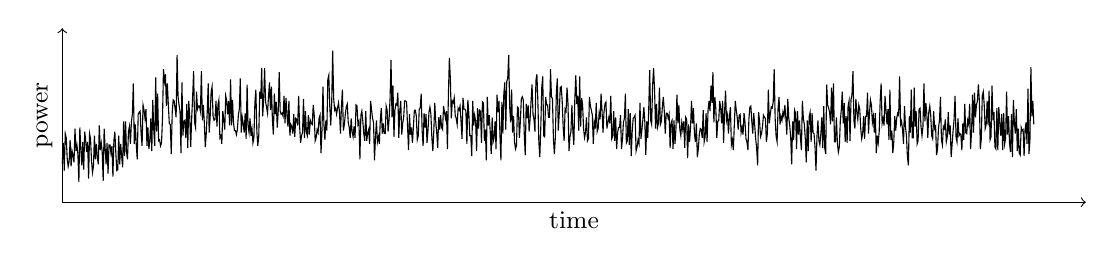
\begin{tikzpicture}[scale=1.3]
      \draw 
(0.000000,-0.120000)
-- (0.010450,0.080000)
-- (0.019950,-0.190000)
-- (0.029450,0.170000)
-- (0.038950,0.130000)
-- (0.048450,-0.070000)
-- (0.057950,-0.150000)
-- (0.067450,-0.100000)
-- (0.076950,0.110000)
-- (0.086450,-0.150000)
-- (0.095950,0.000000)
-- (0.105450,-0.050000)
-- (0.114950,-0.110000)
-- (0.124450,0.220000)
-- (0.133950,0.000000)
-- (0.143450,0.060000)
-- (0.152950,-0.030000)
-- (0.162450,-0.300000)
-- (0.171950,0.230000)
-- (0.181450,0.020000)
-- (0.190950,-0.140000)
-- (0.200450,0.090000)
-- (0.209950,-0.180000)
-- (0.219450,0.190000)
-- (0.228950,0.100000)
-- (0.238450,-0.010000)
-- (0.247950,0.090000)
-- (0.257450,-0.270000)
-- (0.266950,0.170000)
-- (0.276450,0.120000)
-- (0.285950,-0.090000)
-- (0.295450,-0.210000)
-- (0.304950,-0.150000)
-- (0.314450,0.150000)
-- (0.323950,-0.080000)
-- (0.333450,0.070000)
-- (0.342950,-0.060000)
-- (0.352450,-0.130000)
-- (0.361950,0.250000)
-- (0.371450,0.010000)
-- (0.380950,0.080000)
-- (0.390450,-0.010000)
-- (0.399950,-0.290000)
-- (0.409450,0.220000)
-- (0.418950,0.030000)
-- (0.428450,-0.130000)
-- (0.437950,0.080000)
-- (0.447450,-0.220000)
-- (0.456950,0.060000)
-- (0.466450,0.060000)
-- (0.475950,-0.020000)
-- (0.485450,0.050000)
-- (0.494950,-0.250000)
-- (0.504450,0.100000)
-- (0.513950,0.190000)
-- (0.523450,-0.020000)
-- (0.532950,-0.190000)
-- (0.542450,-0.180000)
-- (0.551950,0.150000)
-- (0.561450,-0.130000)
-- (0.570950,0.070000)
-- (0.580450,-0.050000)
-- (0.589950,-0.160000)
-- (0.599450,0.290000)
-- (0.608950,-0.050000)
-- (0.618450,0.290000)
-- (0.627950,-0.010000)
-- (0.637450,-0.080000)
-- (0.646950,0.190000)
-- (0.656450,0.240000)
-- (0.665950,0.070000)
-- (0.675450,0.280000)
-- (0.684950,0.360000)
-- (0.694450,0.660000)
-- (0.703950,0.070000)
-- (0.713450,0.260000)
-- (0.722950,0.070000)
-- (0.732450,-0.080000)
-- (0.741950,0.360000)
-- (0.751450,0.380000)
-- (0.760950,0.390000)
-- (0.770450,0.170000)
-- (0.779950,0.050000)
-- (0.789450,0.450000)
-- (0.798950,0.400000)
-- (0.808450,0.320000)
-- (0.817950,0.410000)
-- (0.827450,0.050000)
-- (0.836950,0.230000)
-- (0.846450,0.020000)
-- (0.855950,0.100000)
-- (0.865450,0.320000)
-- (0.874950,0.000000)
-- (0.884450,0.500000)
-- (0.893950,0.210000)
-- (0.903450,0.050000)
-- (0.912950,0.720000)
-- (0.922450,0.190000)
-- (0.931950,0.560000)
-- (0.941450,0.100000)
-- (0.950950,0.110000)
-- (0.960450,0.050000)
-- (0.969950,0.080000)
-- (0.979450,0.320000)
-- (0.988950,0.800000)
-- (0.998450,0.680000)
-- (1.007950,0.750000)
-- (1.017450,0.440000)
-- (1.026950,0.660000)
-- (1.036450,0.450000)
-- (1.045950,0.270000)
-- (1.055450,0.260000)
-- (1.064950,-0.030000)
-- (1.074450,0.380000)
-- (1.083950,0.500000)
-- (1.093450,0.490000)
-- (1.102950,0.410000)
-- (1.112450,0.330000)
-- (1.121950,0.940000)
-- (1.131450,0.530000)
-- (1.140950,0.450000)
-- (1.150450,0.390000)
-- (1.159950,-0.020000)
-- (1.169450,0.670000)
-- (1.178950,0.150000)
-- (1.188450,0.290000)
-- (1.197950,0.300000)
-- (1.207450,0.130000)
-- (1.216950,0.460000)
-- (1.226450,0.030000)
-- (1.235950,0.490000)
-- (1.245450,0.340000)
-- (1.254950,0.040000)
-- (1.264450,0.320000)
-- (1.273950,0.530000)
-- (1.283450,0.780000)
-- (1.292950,0.280000)
-- (1.302450,0.230000)
-- (1.311950,0.580000)
-- (1.321450,0.410000)
-- (1.330950,0.440000)
-- (1.340450,0.440000)
-- (1.349950,0.390000)
-- (1.359450,0.780000)
-- (1.368950,0.300000)
-- (1.378450,0.450000)
-- (1.387950,0.280000)
-- (1.397450,0.040000)
-- (1.406950,0.170000)
-- (1.416450,0.380000)
-- (1.425950,0.660000)
-- (1.435450,0.180000)
-- (1.444950,0.330000)
-- (1.454450,0.580000)
-- (1.463950,0.630000)
-- (1.473450,0.340000)
-- (1.482950,0.300000)
-- (1.492450,0.310000)
-- (1.501950,0.490000)
-- (1.511450,0.240000)
-- (1.520950,0.450000)
-- (1.530450,0.500000)
-- (1.539950,0.130000)
-- (1.549450,0.150000)
-- (1.558950,0.070000)
-- (1.568450,0.390000)
-- (1.577950,0.310000)
-- (1.587450,0.210000)
-- (1.596950,0.540000)
-- (1.606450,0.490000)
-- (1.615950,0.360000)
-- (1.625450,0.490000)
-- (1.634950,0.250000)
-- (1.644450,0.700000)
-- (1.653950,0.250000)
-- (1.663450,0.500000)
-- (1.672950,0.280000)
-- (1.682450,0.200000)
-- (1.691950,0.200000)
-- (1.701450,0.160000)
-- (1.710950,0.210000)
-- (1.720450,0.350000)
-- (1.729950,0.410000)
-- (1.739450,0.710000)
-- (1.748950,0.180000)
-- (1.758450,0.330000)
-- (1.767950,0.270000)
-- (1.777450,0.180000)
-- (1.786950,0.370000)
-- (1.796450,0.120000)
-- (1.805950,0.650000)
-- (1.815450,0.240000)
-- (1.824950,0.180000)
-- (1.834450,0.320000)
-- (1.843950,0.150000)
-- (1.853450,0.220000)
-- (1.862950,0.080000)
-- (1.872450,0.130000)
-- (1.881950,0.470000)
-- (1.891450,0.600000)
-- (1.900950,0.200000)
-- (1.910450,0.050000)
-- (1.919950,0.150000)
-- (1.929450,0.580000)
-- (1.938950,0.510000)
-- (1.948450,0.810000)
-- (1.957950,0.340000)
-- (1.967450,0.500000)
-- (1.976950,0.810000)
-- (1.986450,0.480000)
-- (1.995950,0.430000)
-- (2.005450,0.370000)
-- (2.014950,0.530000)
-- (2.024450,0.670000)
-- (2.033950,0.400000)
-- (2.043450,0.630000)
-- (2.052950,0.310000)
-- (2.062450,0.160000)
-- (2.071950,0.560000)
-- (2.081450,0.360000)
-- (2.090950,0.480000)
-- (2.100450,0.230000)
-- (2.109950,0.390000)
-- (2.119450,0.770000)
-- (2.128950,0.390000)
-- (2.138450,0.360000)
-- (2.147950,0.370000)
-- (2.157450,0.340000)
-- (2.166950,0.540000)
-- (2.176450,0.270000)
-- (2.185950,0.520000)
-- (2.195450,0.350000)
-- (2.204950,0.240000)
-- (2.214450,0.490000)
-- (2.223950,0.150000)
-- (2.233450,0.260000)
-- (2.242950,0.240000)
-- (2.252450,0.170000)
-- (2.261950,0.360000)
-- (2.271450,0.140000)
-- (2.280950,0.320000)
-- (2.290450,0.310000)
-- (2.299950,0.250000)
-- (2.309450,0.540000)
-- (2.318950,0.240000)
-- (2.328450,0.080000)
-- (2.337950,0.150000)
-- (2.347450,0.180000)
-- (2.356950,0.510000)
-- (2.366450,0.130000)
-- (2.375950,0.390000)
-- (2.385450,0.180000)
-- (2.394950,0.150000)
-- (2.404450,0.350000)
-- (2.413950,0.160000)
-- (2.423450,0.300000)
-- (2.432950,0.270000)
-- (2.442450,0.260000)
-- (2.451950,0.450000)
-- (2.461450,0.350000)
-- (2.470950,0.100000)
-- (2.480450,0.130000)
-- (2.489950,0.210000)
-- (2.499450,0.180000)
-- (2.508950,0.320000)
-- (2.518450,0.350000)
-- (2.527950,-0.020000)
-- (2.537450,0.200000)
-- (2.546950,0.630000)
-- (2.556450,0.260000)
-- (2.565950,0.110000)
-- (2.575450,0.300000)
-- (2.584950,0.200000)
-- (2.594450,0.700000)
-- (2.603950,0.740000)
-- (2.613450,0.440000)
-- (2.622950,0.250000)
-- (2.632450,0.470000)
-- (2.641950,0.980000)
-- (2.651450,0.520000)
-- (2.660950,0.400000)
-- (2.670450,0.420000)
-- (2.679950,0.360000)
-- (2.689450,0.420000)
-- (2.698950,0.470000)
-- (2.708450,0.380000)
-- (2.717950,0.170000)
-- (2.727450,0.430000)
-- (2.736950,0.600000)
-- (2.746450,0.200000)
-- (2.755950,0.260000)
-- (2.765450,0.360000)
-- (2.774950,0.430000)
-- (2.784450,0.460000)
-- (2.793950,0.280000)
-- (2.803450,0.230000)
-- (2.812950,0.130000)
-- (2.822450,0.320000)
-- (2.831950,0.190000)
-- (2.841450,0.140000)
-- (2.850950,0.240000)
-- (2.860450,0.130000)
-- (2.869950,0.450000)
-- (2.879450,0.440000)
-- (2.888950,0.260000)
-- (2.898450,0.290000)
-- (2.907950,-0.080000)
-- (2.917450,0.350000)
-- (2.926950,0.390000)
-- (2.936450,0.290000)
-- (2.945950,0.170000)
-- (2.955450,0.100000)
-- (2.964950,0.390000)
-- (2.974450,0.100000)
-- (2.983950,0.180000)
-- (2.993450,0.210000)
-- (3.002950,0.070000)
-- (3.012450,0.490000)
-- (3.021950,0.400000)
-- (3.031450,0.320000)
-- (3.040950,0.280000)
-- (3.050450,-0.090000)
-- (3.059950,0.130000)
-- (3.069450,0.300000)
-- (3.078950,0.090000)
-- (3.088450,0.140000)
-- (3.097950,0.070000)
-- (3.107450,0.310000)
-- (3.116950,0.420000)
-- (3.126450,0.170000)
-- (3.135950,0.270000)
-- (3.145450,0.170000)
-- (3.154950,0.170000)
-- (3.164450,0.440000)
-- (3.173950,0.400000)
-- (3.183450,0.190000)
-- (3.192950,0.310000)
-- (3.202450,0.510000)
-- (3.211950,0.890000)
-- (3.221450,0.330000)
-- (3.230950,0.640000)
-- (3.240450,0.140000)
-- (3.249950,0.400000)
-- (3.259450,0.460000)
-- (3.268950,0.450000)
-- (3.278450,0.570000)
-- (3.287950,0.130000)
-- (3.297450,0.390000)
-- (3.306950,0.490000)
-- (3.316450,0.160000)
-- (3.325950,0.270000)
-- (3.335450,0.330000)
-- (3.344950,0.490000)
-- (3.354450,0.490000)
-- (3.363950,0.480000)
-- (3.373450,0.240000)
-- (3.382950,0.010000)
-- (3.392450,0.360000)
-- (3.401950,0.160000)
-- (3.411450,0.230000)
-- (3.420950,0.080000)
-- (3.430450,0.230000)
-- (3.439950,0.400000)
-- (3.449450,0.400000)
-- (3.458950,0.340000)
-- (3.468450,0.110000)
-- (3.477950,0.150000)
-- (3.487450,0.410000)
-- (3.496950,0.420000)
-- (3.506450,0.560000)
-- (3.515950,0.200000)
-- (3.525450,0.050000)
-- (3.534950,0.370000)
-- (3.544450,0.230000)
-- (3.553950,0.360000)
-- (3.563450,0.080000)
-- (3.572950,0.200000)
-- (3.582450,0.380000)
-- (3.591950,0.430000)
-- (3.601450,0.360000)
-- (3.610950,0.130000)
-- (3.620450,0.000000)
-- (3.629950,0.200000)
-- (3.639450,0.470000)
-- (3.648950,0.280000)
-- (3.658450,0.180000)
-- (3.667950,0.030000)
-- (3.677450,0.330000)
-- (3.686950,0.210000)
-- (3.696450,0.350000)
-- (3.705950,0.230000)
-- (3.715450,0.210000)
-- (3.724950,0.440000)
-- (3.734450,0.380000)
-- (3.743950,0.320000)
-- (3.753450,0.390000)
-- (3.762950,0.020000)
-- (3.772450,0.550000)
-- (3.781950,0.910000)
-- (3.791450,0.710000)
-- (3.800950,0.320000)
-- (3.810450,0.490000)
-- (3.819950,0.470000)
-- (3.829450,0.520000)
-- (3.838950,0.350000)
-- (3.848450,0.320000)
-- (3.857950,0.260000)
-- (3.867450,0.420000)
-- (3.876950,0.400000)
-- (3.886450,0.440000)
-- (3.895950,0.290000)
-- (3.905450,0.120000)
-- (3.914950,0.520000)
-- (3.924450,0.410000)
-- (3.933950,0.410000)
-- (3.943450,0.390000)
-- (3.952950,0.070000)
-- (3.962450,0.500000)
-- (3.971950,0.370000)
-- (3.981450,0.150000)
-- (3.990950,0.150000)
-- (4.000450,-0.050000)
-- (4.009950,0.490000)
-- (4.019450,0.250000)
-- (4.028950,0.350000)
-- (4.038450,0.290000)
-- (4.047950,0.000000)
-- (4.057450,0.420000)
-- (4.066950,0.220000)
-- (4.076450,0.400000)
-- (4.085950,0.390000)
-- (4.095450,0.080000)
-- (4.104950,0.480000)
-- (4.114450,0.470000)
-- (4.123950,0.100000)
-- (4.133450,0.210000)
-- (4.142950,-0.090000)
-- (4.152450,0.530000)
-- (4.161950,0.250000)
-- (4.171450,0.350000)
-- (4.180950,0.190000)
-- (4.190450,-0.030000)
-- (4.199950,0.330000)
-- (4.209450,0.090000)
-- (4.218950,0.130000)
-- (4.228450,0.290000)
-- (4.237950,0.020000)
-- (4.247450,0.550000)
-- (4.256950,0.380000)
-- (4.266450,0.490000)
-- (4.275950,0.160000)
-- (4.285450,-0.090000)
-- (4.294950,0.480000)
-- (4.304450,0.170000)
-- (4.313950,0.560000)
-- (4.323450,0.670000)
-- (4.332950,0.210000)
-- (4.342450,0.680000)
-- (4.351950,0.710000)
-- (4.361450,0.940000)
-- (4.370950,0.430000)
-- (4.380450,0.280000)
-- (4.389950,0.600000)
-- (4.399450,0.180000)
-- (4.408950,0.340000)
-- (4.418450,0.090000)
-- (4.427950,0.020000)
-- (4.437450,0.050000)
-- (4.446950,0.430000)
-- (4.456450,0.420000)
-- (4.465950,0.130000)
-- (4.475450,0.290000)
-- (4.484950,0.510000)
-- (4.494450,0.530000)
-- (4.503950,0.500000)
-- (4.513450,0.170000)
-- (4.522950,-0.040000)
-- (4.532450,0.460000)
-- (4.541950,0.320000)
-- (4.551450,0.450000)
-- (4.560950,0.190000)
-- (4.570450,0.310000)
-- (4.579950,0.490000)
-- (4.589450,0.650000)
-- (4.598950,0.360000)
-- (4.608450,0.310000)
-- (4.617950,0.190000)
-- (4.627450,0.690000)
-- (4.636950,0.750000)
-- (4.646450,0.490000)
-- (4.655950,0.090000)
-- (4.665450,-0.060000)
-- (4.674950,0.230000)
-- (4.684450,0.620000)
-- (4.693950,0.730000)
-- (4.703450,0.150000)
-- (4.712950,0.140000)
-- (4.722450,0.530000)
-- (4.731950,0.450000)
-- (4.741450,0.450000)
-- (4.750950,0.330000)
-- (4.760450,0.330000)
-- (4.769950,0.800000)
-- (4.779450,0.530000)
-- (4.788950,0.510000)
-- (4.798450,0.120000)
-- (4.807950,-0.030000)
-- (4.817450,0.140000)
-- (4.826950,0.570000)
-- (4.836450,0.710000)
-- (4.845950,0.200000)
-- (4.855450,0.370000)
-- (4.864950,0.620000)
-- (4.874450,0.630000)
-- (4.883950,0.490000)
-- (4.893450,0.240000)
-- (4.902950,0.100000)
-- (4.912450,0.410000)
-- (4.921950,0.390000)
-- (4.931450,0.620000)
-- (4.940950,0.460000)
-- (4.950450,0.000000)
-- (4.959950,0.140000)
-- (4.969450,0.190000)
-- (4.978950,0.450000)
-- (4.988450,0.190000)
-- (4.997950,0.060000)
-- (5.007450,0.510000)
-- (5.016950,0.740000)
-- (5.026450,0.460000)
-- (5.035950,0.540000)
-- (5.045450,0.200000)
-- (5.054950,0.730000)
-- (5.064450,0.240000)
-- (5.073950,0.520000)
-- (5.083450,0.450000)
-- (5.092950,0.220000)
-- (5.102450,0.130000)
-- (5.111950,0.180000)
-- (5.121450,0.330000)
-- (5.130950,0.100000)
-- (5.140450,0.120000)
-- (5.149950,0.530000)
-- (5.159450,0.440000)
-- (5.168950,0.400000)
-- (5.178450,0.350000)
-- (5.187950,0.070000)
-- (5.197450,0.280000)
-- (5.206950,0.220000)
-- (5.216450,0.470000)
-- (5.225950,0.190000)
-- (5.235450,0.220000)
-- (5.244950,0.370000)
-- (5.254450,0.310000)
-- (5.263950,0.560000)
-- (5.273450,0.390000)
-- (5.282950,0.180000)
-- (5.292450,0.380000)
-- (5.301950,0.460000)
-- (5.311450,0.480000)
-- (5.320950,0.220000)
-- (5.330450,0.280000)
-- (5.339950,0.330000)
-- (5.349450,0.270000)
-- (5.358950,0.540000)
-- (5.368450,0.120000)
-- (5.377950,0.150000)
-- (5.387450,0.390000)
-- (5.396950,0.100000)
-- (5.406450,0.330000)
-- (5.415950,0.020000)
-- (5.425450,0.180000)
-- (5.434950,0.230000)
-- (5.444450,0.230000)
-- (5.453950,0.350000)
-- (5.463450,0.020000)
-- (5.472950,0.120000)
-- (5.482450,0.280000)
-- (5.491950,0.320000)
-- (5.501450,0.560000)
-- (5.510950,0.080000)
-- (5.520450,0.100000)
-- (5.529950,0.410000)
-- (5.539450,0.060000)
-- (5.548950,0.370000)
-- (5.558450,-0.050000)
-- (5.567950,0.190000)
-- (5.577450,0.320000)
-- (5.586950,0.330000)
-- (5.596450,0.350000)
-- (5.605950,0.000000)
-- (5.615450,0.040000)
-- (5.624950,0.110000)
-- (5.634450,0.070000)
-- (5.643950,0.470000)
-- (5.653450,0.120000)
-- (5.662950,0.210000)
-- (5.672450,0.310000)
-- (5.681950,0.430000)
-- (5.691450,0.280000)
-- (5.700950,-0.040000)
-- (5.710450,0.290000)
-- (5.719950,0.130000)
-- (5.729450,0.410000)
-- (5.738950,0.790000)
-- (5.748450,0.300000)
-- (5.757950,0.260000)
-- (5.767450,0.640000)
-- (5.776950,0.810000)
-- (5.786450,0.600000)
-- (5.795950,0.220000)
-- (5.805450,0.460000)
-- (5.814950,0.230000)
-- (5.824450,0.270000)
-- (5.833950,0.620000)
-- (5.843450,0.260000)
-- (5.852950,0.290000)
-- (5.862450,0.430000)
-- (5.871950,0.530000)
-- (5.881450,0.390000)
-- (5.890950,0.170000)
-- (5.900450,0.370000)
-- (5.909950,0.370000)
-- (5.919450,0.320000)
-- (5.928950,0.360000)
-- (5.938450,0.030000)
-- (5.947950,0.280000)
-- (5.957450,0.300000)
-- (5.966950,0.020000)
-- (5.976450,0.300000)
-- (5.985950,0.070000)
-- (5.995450,0.220000)
-- (6.004950,0.550000)
-- (6.014450,0.270000)
-- (6.023950,0.450000)
-- (6.033450,0.210000)
-- (6.042950,0.150000)
-- (6.052450,0.280000)
-- (6.061950,0.210000)
-- (6.071450,0.290000)
-- (6.080950,0.030000)
-- (6.090450,0.330000)
-- (6.099950,0.310000)
-- (6.109450,-0.070000)
-- (6.118950,0.260000)
-- (6.128450,0.090000)
-- (6.137950,0.230000)
-- (6.147450,0.490000)
-- (6.156950,0.270000)
-- (6.166450,0.420000)
-- (6.175950,0.170000)
-- (6.185450,0.090000)
-- (6.194950,0.270000)
-- (6.204450,-0.060000)
-- (6.213950,0.020000)
-- (6.223450,0.160000)
-- (6.232950,0.220000)
-- (6.242450,0.210000)
-- (6.251950,0.130000)
-- (6.261450,0.400000)
-- (6.270950,0.090000)
-- (6.280450,0.140000)
-- (6.289950,0.370000)
-- (6.299450,0.090000)
-- (6.308950,0.400000)
-- (6.318450,0.490000)
-- (6.327950,0.390000)
-- (6.337450,0.640000)
-- (6.346950,0.470000)
-- (6.356450,0.770000)
-- (6.365950,0.280000)
-- (6.375450,0.530000)
-- (6.384950,0.410000)
-- (6.394450,0.130000)
-- (6.403950,0.290000)
-- (6.413450,0.300000)
-- (6.422950,0.490000)
-- (6.432450,0.420000)
-- (6.441950,0.270000)
-- (6.451450,0.490000)
-- (6.460950,0.080000)
-- (6.470450,0.380000)
-- (6.479950,0.590000)
-- (6.489450,0.300000)
-- (6.498950,0.350000)
-- (6.508450,0.170000)
-- (6.517950,0.340000)
-- (6.527450,0.430000)
-- (6.536950,0.060000)
-- (6.546450,0.110000)
-- (6.555950,0.010000)
-- (6.565450,0.250000)
-- (6.574950,0.490000)
-- (6.584450,0.400000)
-- (6.593950,0.330000)
-- (6.603450,0.210000)
-- (6.612950,0.350000)
-- (6.622450,0.360000)
-- (6.631950,0.180000)
-- (6.641450,0.230000)
-- (6.650950,0.160000)
-- (6.660450,0.370000)
-- (6.669950,0.280000)
-- (6.679450,0.120000)
-- (6.688950,0.090000)
-- (6.698450,0.010000)
-- (6.707950,0.310000)
-- (6.717450,0.430000)
-- (6.726950,0.440000)
-- (6.736450,0.290000)
-- (6.745950,0.170000)
-- (6.755450,0.370000)
-- (6.764950,0.250000)
-- (6.774450,0.120000)
-- (6.783950,0.020000)
-- (6.793450,-0.140000)
-- (6.802950,0.380000)
-- (6.812450,0.290000)
-- (6.821950,0.140000)
-- (6.831450,0.170000)
-- (6.840950,0.240000)
-- (6.850450,0.350000)
-- (6.859950,0.330000)
-- (6.869450,0.320000)
-- (6.878950,0.090000)
-- (6.888450,0.170000)
-- (6.897950,0.600000)
-- (6.907450,0.270000)
-- (6.916950,0.360000)
-- (6.926450,0.430000)
-- (6.935950,0.420000)
-- (6.945450,0.480000)
-- (6.954950,0.800000)
-- (6.964450,0.320000)
-- (6.973950,0.140000)
-- (6.983450,0.090000)
-- (6.992950,0.420000)
-- (7.002450,0.530000)
-- (7.011950,0.260000)
-- (7.021450,0.340000)
-- (7.030950,0.300000)
-- (7.040450,0.380000)
-- (7.049950,0.340000)
-- (7.059450,0.450000)
-- (7.068950,0.320000)
-- (7.078450,0.160000)
-- (7.087950,0.510000)
-- (7.097450,0.320000)
-- (7.106950,0.250000)
-- (7.116450,0.130000)
-- (7.125950,-0.130000)
-- (7.135450,0.290000)
-- (7.144950,0.110000)
-- (7.154450,0.400000)
-- (7.163950,0.370000)
-- (7.173450,0.020000)
-- (7.182950,0.390000)
-- (7.192450,0.160000)
-- (7.201950,0.300000)
-- (7.211450,0.130000)
-- (7.220950,0.010000)
-- (7.230450,0.490000)
-- (7.239950,0.320000)
-- (7.249450,0.260000)
-- (7.258950,0.120000)
-- (7.268450,-0.110000)
-- (7.277950,0.300000)
-- (7.287450,0.000000)
-- (7.296950,0.340000)
-- (7.306450,0.380000)
-- (7.315950,0.090000)
-- (7.325450,0.370000)
-- (7.334950,0.180000)
-- (7.344450,0.170000)
-- (7.353950,0.040000)
-- (7.363450,-0.190000)
-- (7.372950,0.140000)
-- (7.382450,0.300000)
-- (7.391950,0.100000)
-- (7.401450,0.060000)
-- (7.410950,0.170000)
-- (7.420450,0.330000)
-- (7.429950,0.030000)
-- (7.439450,0.440000)
-- (7.448950,0.030000)
-- (7.458450,-0.030000)
-- (7.467950,0.650000)
-- (7.477450,0.450000)
-- (7.486950,0.420000)
-- (7.496450,0.380000)
-- (7.505950,0.260000)
-- (7.515450,0.620000)
-- (7.524950,0.290000)
-- (7.534450,0.660000)
-- (7.543950,0.090000)
-- (7.553450,0.090000)
-- (7.562950,0.330000)
-- (7.572450,0.080000)
-- (7.581950,-0.010000)
-- (7.591450,0.040000)
-- (7.600950,0.290000)
-- (7.610450,0.400000)
-- (7.619950,0.580000)
-- (7.629450,0.270000)
-- (7.638950,0.470000)
-- (7.648450,0.090000)
-- (7.657950,0.340000)
-- (7.667450,0.080000)
-- (7.676950,0.440000)
-- (7.686450,0.490000)
-- (7.695950,0.100000)
-- (7.705450,0.500000)
-- (7.714950,0.550000)
-- (7.724450,0.780000)
-- (7.733950,0.300000)
-- (7.743450,0.220000)
-- (7.752950,0.510000)
-- (7.762450,0.380000)
-- (7.771950,0.310000)
-- (7.781450,0.450000)
-- (7.790950,0.410000)
-- (7.800450,0.220000)
-- (7.809950,0.120000)
-- (7.819450,0.170000)
-- (7.828950,0.340000)
-- (7.838450,0.120000)
-- (7.847950,0.340000)
-- (7.857450,0.340000)
-- (7.866950,0.570000)
-- (7.876450,0.170000)
-- (7.885950,0.370000)
-- (7.895450,0.500000)
-- (7.904950,0.450000)
-- (7.914450,0.280000)
-- (7.923950,0.340000)
-- (7.933450,0.180000)
-- (7.942950,0.370000)
-- (7.952450,-0.020000)
-- (7.961950,0.150000)
-- (7.971450,0.080000)
-- (7.980950,0.190000)
-- (7.990450,0.490000)
-- (7.999950,0.660000)
-- (8.009450,0.270000)
-- (8.018950,0.320000)
-- (8.028450,0.250000)
-- (8.037950,0.540000)
-- (8.047450,0.400000)
-- (8.056950,0.260000)
-- (8.066450,0.410000)
-- (8.075950,0.110000)
-- (8.085450,0.600000)
-- (8.094950,0.110000)
-- (8.104450,0.200000)
-- (8.113950,-0.020000)
-- (8.123450,0.090000)
-- (8.132950,0.340000)
-- (8.142450,0.200000)
-- (8.151950,0.320000)
-- (8.161450,0.370000)
-- (8.170950,0.350000)
-- (8.180450,0.730000)
-- (8.189950,0.260000)
-- (8.199450,0.290000)
-- (8.208950,0.210000)
-- (8.218450,0.070000)
-- (8.227950,0.440000)
-- (8.237450,0.240000)
-- (8.246950,0.150000)
-- (8.256450,-0.050000)
-- (8.265950,-0.140000)
-- (8.275450,0.340000)
-- (8.284950,0.180000)
-- (8.294450,0.600000)
-- (8.303950,0.130000)
-- (8.313450,0.130000)
-- (8.322950,0.620000)
-- (8.332450,0.240000)
-- (8.341950,0.390000)
-- (8.351450,0.070000)
-- (8.360950,0.100000)
-- (8.370450,0.410000)
-- (8.379950,0.420000)
-- (8.389450,0.240000)
-- (8.398950,0.150000)
-- (8.408450,0.240000)
-- (8.417950,0.660000)
-- (8.427450,0.290000)
-- (8.436950,0.470000)
-- (8.446450,0.360000)
-- (8.455950,0.130000)
-- (8.465450,0.380000)
-- (8.474950,0.440000)
-- (8.484450,0.350000)
-- (8.493950,0.150000)
-- (8.503450,0.120000)
-- (8.512950,0.390000)
-- (8.522450,0.220000)
-- (8.531950,0.240000)
-- (8.541450,-0.040000)
-- (8.550950,0.020000)
-- (8.560450,0.230000)
-- (8.569950,0.300000)
-- (8.579450,0.530000)
-- (8.588950,0.110000)
-- (8.598450,0.060000)
-- (8.607950,0.240000)
-- (8.617450,0.220000)
-- (8.626950,0.310000)
-- (8.636450,0.090000)
-- (8.645950,0.140000)
-- (8.655450,0.380000)
-- (8.664950,0.160000)
-- (8.674450,0.250000)
-- (8.683950,-0.060000)
-- (8.693450,0.070000)
-- (8.702950,0.200000)
-- (8.712450,0.310000)
-- (8.721950,0.540000)
-- (8.731450,0.140000)
-- (8.740950,0.090000)
-- (8.750450,0.320000)
-- (8.759950,0.150000)
-- (8.769450,0.170000)
-- (8.778950,0.160000)
-- (8.788450,0.010000)
-- (8.797950,0.270000)
-- (8.807450,0.110000)
-- (8.816950,0.460000)
-- (8.826450,0.180000)
-- (8.835950,0.170000)
-- (8.845450,0.300000)
-- (8.854950,0.260000)
-- (8.864450,0.460000)
-- (8.873950,0.020000)
-- (8.883450,0.200000)
-- (8.892950,0.550000)
-- (8.902450,0.180000)
-- (8.911950,0.570000)
-- (8.921450,0.330000)
-- (8.930950,0.450000)
-- (8.940450,0.490000)
-- (8.949950,0.650000)
-- (8.959450,0.490000)
-- (8.968950,0.020000)
-- (8.978450,0.120000)
-- (8.987950,0.540000)
-- (8.997450,0.580000)
-- (9.006950,0.450000)
-- (9.016450,0.220000)
-- (9.025950,0.260000)
-- (9.035450,0.490000)
-- (9.044950,0.250000)
-- (9.054450,0.590000)
-- (9.063950,0.110000)
-- (9.073450,0.140000)
-- (9.082950,0.640000)
-- (9.092450,0.300000)
-- (9.101950,0.380000)
-- (9.111450,0.040000)
-- (9.120950,0.020000)
-- (9.130450,0.420000)
-- (9.139950,0.010000)
-- (9.149450,0.430000)
-- (9.158950,0.270000)
-- (9.168450,0.150000)
-- (9.177950,0.360000)
-- (9.187450,0.010000)
-- (9.196950,0.370000)
-- (9.206450,0.070000)
-- (9.215950,0.120000)
-- (9.225450,0.580000)
-- (9.234950,0.160000)
-- (9.244450,0.340000)
-- (9.253950,0.080000)
-- (9.263450,-0.010000)
-- (9.272950,0.360000)
-- (9.282450,-0.060000)
-- (9.291950,0.500000)
-- (9.301450,0.280000)
-- (9.310950,0.170000)
-- (9.320450,0.410000)
-- (9.329950,0.000000)
-- (9.339450,0.220000)
-- (9.348950,-0.020000)
-- (9.358450,-0.040000)
-- (9.367950,0.230000)
-- (9.377450,0.200000)
-- (9.386950,0.210000)
-- (9.396450,-0.050000)
-- (9.405950,0.210000)
-- (9.415450,0.280000)
-- (9.424950,0.070000)
-- (9.434450,0.610000)
-- (9.443950,-0.030000)
-- (9.453450,0.100000)
-- (9.462950,0.820000)
-- (9.472450,0.340000)
-- (9.481950,0.490000)
-- (9.491450,0.260000)
;

      \draw[->] (0,-.5) -- (0,1.2) node[midway, above,rotate=90] {\small{power}};
      \draw[->] (0,-.5) -- (10,-.5) node[midway, below] {\small{time}};
    \end{tikzpicture}
  \end{figure}

  \begin{block}{Traces as functions}
    Power traces are functions over time, with constant input
  \end{block}
  \vfill
\end{frame}

\begin{frame}[label=traces]
  \frametitle{Power analysis cont.}
  \begin{figure}
    \begin{tikzpicture}
      \draw<2->[draw=uibkorange, fill=uibkorangel] (3.05,1) rectangle (3.15,-4.8);
      \node<2-> at (3.1, -5.1) {\textcolor{uibkorange}{Function over input, at constant time}};
      \begin{scope}
        \node at (-1.2, .4) {$\textup{Input}_1$};
        \draw 
(0.000000,-0.120000)
-- (0.010450,0.080000)
-- (0.019950,-0.190000)
-- (0.029450,0.170000)
-- (0.038950,0.130000)
-- (0.048450,-0.070000)
-- (0.057950,-0.150000)
-- (0.067450,-0.100000)
-- (0.076950,0.110000)
-- (0.086450,-0.150000)
-- (0.095950,0.000000)
-- (0.105450,-0.050000)
-- (0.114950,-0.110000)
-- (0.124450,0.220000)
-- (0.133950,0.000000)
-- (0.143450,0.060000)
-- (0.152950,-0.030000)
-- (0.162450,-0.300000)
-- (0.171950,0.230000)
-- (0.181450,0.020000)
-- (0.190950,-0.140000)
-- (0.200450,0.090000)
-- (0.209950,-0.180000)
-- (0.219450,0.190000)
-- (0.228950,0.100000)
-- (0.238450,-0.010000)
-- (0.247950,0.090000)
-- (0.257450,-0.270000)
-- (0.266950,0.170000)
-- (0.276450,0.120000)
-- (0.285950,-0.090000)
-- (0.295450,-0.210000)
-- (0.304950,-0.150000)
-- (0.314450,0.150000)
-- (0.323950,-0.080000)
-- (0.333450,0.070000)
-- (0.342950,-0.060000)
-- (0.352450,-0.130000)
-- (0.361950,0.250000)
-- (0.371450,0.010000)
-- (0.380950,0.080000)
-- (0.390450,-0.010000)
-- (0.399950,-0.290000)
-- (0.409450,0.220000)
-- (0.418950,0.030000)
-- (0.428450,-0.130000)
-- (0.437950,0.080000)
-- (0.447450,-0.220000)
-- (0.456950,0.060000)
-- (0.466450,0.060000)
-- (0.475950,-0.020000)
-- (0.485450,0.050000)
-- (0.494950,-0.250000)
-- (0.504450,0.100000)
-- (0.513950,0.190000)
-- (0.523450,-0.020000)
-- (0.532950,-0.190000)
-- (0.542450,-0.180000)
-- (0.551950,0.150000)
-- (0.561450,-0.130000)
-- (0.570950,0.070000)
-- (0.580450,-0.050000)
-- (0.589950,-0.160000)
-- (0.599450,0.290000)
-- (0.608950,-0.050000)
-- (0.618450,0.290000)
-- (0.627950,-0.010000)
-- (0.637450,-0.080000)
-- (0.646950,0.190000)
-- (0.656450,0.240000)
-- (0.665950,0.070000)
-- (0.675450,0.280000)
-- (0.684950,0.360000)
-- (0.694450,0.660000)
-- (0.703950,0.070000)
-- (0.713450,0.260000)
-- (0.722950,0.070000)
-- (0.732450,-0.080000)
-- (0.741950,0.360000)
-- (0.751450,0.380000)
-- (0.760950,0.390000)
-- (0.770450,0.170000)
-- (0.779950,0.050000)
-- (0.789450,0.450000)
-- (0.798950,0.400000)
-- (0.808450,0.320000)
-- (0.817950,0.410000)
-- (0.827450,0.050000)
-- (0.836950,0.230000)
-- (0.846450,0.020000)
-- (0.855950,0.100000)
-- (0.865450,0.320000)
-- (0.874950,0.000000)
-- (0.884450,0.500000)
-- (0.893950,0.210000)
-- (0.903450,0.050000)
-- (0.912950,0.720000)
-- (0.922450,0.190000)
-- (0.931950,0.560000)
-- (0.941450,0.100000)
-- (0.950950,0.110000)
-- (0.960450,0.050000)
-- (0.969950,0.080000)
-- (0.979450,0.320000)
-- (0.988950,0.800000)
-- (0.998450,0.680000)
-- (1.007950,0.750000)
-- (1.017450,0.440000)
-- (1.026950,0.660000)
-- (1.036450,0.450000)
-- (1.045950,0.270000)
-- (1.055450,0.260000)
-- (1.064950,-0.030000)
-- (1.074450,0.380000)
-- (1.083950,0.500000)
-- (1.093450,0.490000)
-- (1.102950,0.410000)
-- (1.112450,0.330000)
-- (1.121950,0.940000)
-- (1.131450,0.530000)
-- (1.140950,0.450000)
-- (1.150450,0.390000)
-- (1.159950,-0.020000)
-- (1.169450,0.670000)
-- (1.178950,0.150000)
-- (1.188450,0.290000)
-- (1.197950,0.300000)
-- (1.207450,0.130000)
-- (1.216950,0.460000)
-- (1.226450,0.030000)
-- (1.235950,0.490000)
-- (1.245450,0.340000)
-- (1.254950,0.040000)
-- (1.264450,0.320000)
-- (1.273950,0.530000)
-- (1.283450,0.780000)
-- (1.292950,0.280000)
-- (1.302450,0.230000)
-- (1.311950,0.580000)
-- (1.321450,0.410000)
-- (1.330950,0.440000)
-- (1.340450,0.440000)
-- (1.349950,0.390000)
-- (1.359450,0.780000)
-- (1.368950,0.300000)
-- (1.378450,0.450000)
-- (1.387950,0.280000)
-- (1.397450,0.040000)
-- (1.406950,0.170000)
-- (1.416450,0.380000)
-- (1.425950,0.660000)
-- (1.435450,0.180000)
-- (1.444950,0.330000)
-- (1.454450,0.580000)
-- (1.463950,0.630000)
-- (1.473450,0.340000)
-- (1.482950,0.300000)
-- (1.492450,0.310000)
-- (1.501950,0.490000)
-- (1.511450,0.240000)
-- (1.520950,0.450000)
-- (1.530450,0.500000)
-- (1.539950,0.130000)
-- (1.549450,0.150000)
-- (1.558950,0.070000)
-- (1.568450,0.390000)
-- (1.577950,0.310000)
-- (1.587450,0.210000)
-- (1.596950,0.540000)
-- (1.606450,0.490000)
-- (1.615950,0.360000)
-- (1.625450,0.490000)
-- (1.634950,0.250000)
-- (1.644450,0.700000)
-- (1.653950,0.250000)
-- (1.663450,0.500000)
-- (1.672950,0.280000)
-- (1.682450,0.200000)
-- (1.691950,0.200000)
-- (1.701450,0.160000)
-- (1.710950,0.210000)
-- (1.720450,0.350000)
-- (1.729950,0.410000)
-- (1.739450,0.710000)
-- (1.748950,0.180000)
-- (1.758450,0.330000)
-- (1.767950,0.270000)
-- (1.777450,0.180000)
-- (1.786950,0.370000)
-- (1.796450,0.120000)
-- (1.805950,0.650000)
-- (1.815450,0.240000)
-- (1.824950,0.180000)
-- (1.834450,0.320000)
-- (1.843950,0.150000)
-- (1.853450,0.220000)
-- (1.862950,0.080000)
-- (1.872450,0.130000)
-- (1.881950,0.470000)
-- (1.891450,0.600000)
-- (1.900950,0.200000)
-- (1.910450,0.050000)
-- (1.919950,0.150000)
-- (1.929450,0.580000)
-- (1.938950,0.510000)
-- (1.948450,0.810000)
-- (1.957950,0.340000)
-- (1.967450,0.500000)
-- (1.976950,0.810000)
-- (1.986450,0.480000)
-- (1.995950,0.430000)
-- (2.005450,0.370000)
-- (2.014950,0.530000)
-- (2.024450,0.670000)
-- (2.033950,0.400000)
-- (2.043450,0.630000)
-- (2.052950,0.310000)
-- (2.062450,0.160000)
-- (2.071950,0.560000)
-- (2.081450,0.360000)
-- (2.090950,0.480000)
-- (2.100450,0.230000)
-- (2.109950,0.390000)
-- (2.119450,0.770000)
-- (2.128950,0.390000)
-- (2.138450,0.360000)
-- (2.147950,0.370000)
-- (2.157450,0.340000)
-- (2.166950,0.540000)
-- (2.176450,0.270000)
-- (2.185950,0.520000)
-- (2.195450,0.350000)
-- (2.204950,0.240000)
-- (2.214450,0.490000)
-- (2.223950,0.150000)
-- (2.233450,0.260000)
-- (2.242950,0.240000)
-- (2.252450,0.170000)
-- (2.261950,0.360000)
-- (2.271450,0.140000)
-- (2.280950,0.320000)
-- (2.290450,0.310000)
-- (2.299950,0.250000)
-- (2.309450,0.540000)
-- (2.318950,0.240000)
-- (2.328450,0.080000)
-- (2.337950,0.150000)
-- (2.347450,0.180000)
-- (2.356950,0.510000)
-- (2.366450,0.130000)
-- (2.375950,0.390000)
-- (2.385450,0.180000)
-- (2.394950,0.150000)
-- (2.404450,0.350000)
-- (2.413950,0.160000)
-- (2.423450,0.300000)
-- (2.432950,0.270000)
-- (2.442450,0.260000)
-- (2.451950,0.450000)
-- (2.461450,0.350000)
-- (2.470950,0.100000)
-- (2.480450,0.130000)
-- (2.489950,0.210000)
-- (2.499450,0.180000)
-- (2.508950,0.320000)
-- (2.518450,0.350000)
-- (2.527950,-0.020000)
-- (2.537450,0.200000)
-- (2.546950,0.630000)
-- (2.556450,0.260000)
-- (2.565950,0.110000)
-- (2.575450,0.300000)
-- (2.584950,0.200000)
-- (2.594450,0.700000)
-- (2.603950,0.740000)
-- (2.613450,0.440000)
-- (2.622950,0.250000)
-- (2.632450,0.470000)
-- (2.641950,0.980000)
-- (2.651450,0.520000)
-- (2.660950,0.400000)
-- (2.670450,0.420000)
-- (2.679950,0.360000)
-- (2.689450,0.420000)
-- (2.698950,0.470000)
-- (2.708450,0.380000)
-- (2.717950,0.170000)
-- (2.727450,0.430000)
-- (2.736950,0.600000)
-- (2.746450,0.200000)
-- (2.755950,0.260000)
-- (2.765450,0.360000)
-- (2.774950,0.430000)
-- (2.784450,0.460000)
-- (2.793950,0.280000)
-- (2.803450,0.230000)
-- (2.812950,0.130000)
-- (2.822450,0.320000)
-- (2.831950,0.190000)
-- (2.841450,0.140000)
-- (2.850950,0.240000)
-- (2.860450,0.130000)
-- (2.869950,0.450000)
-- (2.879450,0.440000)
-- (2.888950,0.260000)
-- (2.898450,0.290000)
-- (2.907950,-0.080000)
-- (2.917450,0.350000)
-- (2.926950,0.390000)
-- (2.936450,0.290000)
-- (2.945950,0.170000)
-- (2.955450,0.100000)
-- (2.964950,0.390000)
-- (2.974450,0.100000)
-- (2.983950,0.180000)
-- (2.993450,0.210000)
-- (3.002950,0.070000)
-- (3.012450,0.490000)
-- (3.021950,0.400000)
-- (3.031450,0.320000)
-- (3.040950,0.280000)
-- (3.050450,-0.090000)
-- (3.059950,0.130000)
-- (3.069450,0.300000)
-- (3.078950,0.090000)
-- (3.088450,0.140000)
-- (3.097950,0.070000)
-- (3.107450,0.310000)
-- (3.116950,0.420000)
-- (3.126450,0.170000)
-- (3.135950,0.270000)
-- (3.145450,0.170000)
-- (3.154950,0.170000)
-- (3.164450,0.440000)
-- (3.173950,0.400000)
-- (3.183450,0.190000)
-- (3.192950,0.310000)
-- (3.202450,0.510000)
-- (3.211950,0.890000)
-- (3.221450,0.330000)
-- (3.230950,0.640000)
-- (3.240450,0.140000)
-- (3.249950,0.400000)
-- (3.259450,0.460000)
-- (3.268950,0.450000)
-- (3.278450,0.570000)
-- (3.287950,0.130000)
-- (3.297450,0.390000)
-- (3.306950,0.490000)
-- (3.316450,0.160000)
-- (3.325950,0.270000)
-- (3.335450,0.330000)
-- (3.344950,0.490000)
-- (3.354450,0.490000)
-- (3.363950,0.480000)
-- (3.373450,0.240000)
-- (3.382950,0.010000)
-- (3.392450,0.360000)
-- (3.401950,0.160000)
-- (3.411450,0.230000)
-- (3.420950,0.080000)
-- (3.430450,0.230000)
-- (3.439950,0.400000)
-- (3.449450,0.400000)
-- (3.458950,0.340000)
-- (3.468450,0.110000)
-- (3.477950,0.150000)
-- (3.487450,0.410000)
-- (3.496950,0.420000)
-- (3.506450,0.560000)
-- (3.515950,0.200000)
-- (3.525450,0.050000)
-- (3.534950,0.370000)
-- (3.544450,0.230000)
-- (3.553950,0.360000)
-- (3.563450,0.080000)
-- (3.572950,0.200000)
-- (3.582450,0.380000)
-- (3.591950,0.430000)
-- (3.601450,0.360000)
-- (3.610950,0.130000)
-- (3.620450,0.000000)
-- (3.629950,0.200000)
-- (3.639450,0.470000)
-- (3.648950,0.280000)
-- (3.658450,0.180000)
-- (3.667950,0.030000)
-- (3.677450,0.330000)
-- (3.686950,0.210000)
-- (3.696450,0.350000)
-- (3.705950,0.230000)
-- (3.715450,0.210000)
-- (3.724950,0.440000)
-- (3.734450,0.380000)
-- (3.743950,0.320000)
-- (3.753450,0.390000)
-- (3.762950,0.020000)
-- (3.772450,0.550000)
-- (3.781950,0.910000)
-- (3.791450,0.710000)
-- (3.800950,0.320000)
-- (3.810450,0.490000)
-- (3.819950,0.470000)
-- (3.829450,0.520000)
-- (3.838950,0.350000)
-- (3.848450,0.320000)
-- (3.857950,0.260000)
-- (3.867450,0.420000)
-- (3.876950,0.400000)
-- (3.886450,0.440000)
-- (3.895950,0.290000)
-- (3.905450,0.120000)
-- (3.914950,0.520000)
-- (3.924450,0.410000)
-- (3.933950,0.410000)
-- (3.943450,0.390000)
-- (3.952950,0.070000)
-- (3.962450,0.500000)
-- (3.971950,0.370000)
-- (3.981450,0.150000)
-- (3.990950,0.150000)
-- (4.000450,-0.050000)
-- (4.009950,0.490000)
-- (4.019450,0.250000)
-- (4.028950,0.350000)
-- (4.038450,0.290000)
-- (4.047950,0.000000)
-- (4.057450,0.420000)
-- (4.066950,0.220000)
-- (4.076450,0.400000)
-- (4.085950,0.390000)
-- (4.095450,0.080000)
-- (4.104950,0.480000)
-- (4.114450,0.470000)
-- (4.123950,0.100000)
-- (4.133450,0.210000)
-- (4.142950,-0.090000)
-- (4.152450,0.530000)
-- (4.161950,0.250000)
-- (4.171450,0.350000)
-- (4.180950,0.190000)
-- (4.190450,-0.030000)
-- (4.199950,0.330000)
-- (4.209450,0.090000)
-- (4.218950,0.130000)
-- (4.228450,0.290000)
-- (4.237950,0.020000)
-- (4.247450,0.550000)
-- (4.256950,0.380000)
-- (4.266450,0.490000)
-- (4.275950,0.160000)
-- (4.285450,-0.090000)
-- (4.294950,0.480000)
-- (4.304450,0.170000)
-- (4.313950,0.560000)
-- (4.323450,0.670000)
-- (4.332950,0.210000)
-- (4.342450,0.680000)
-- (4.351950,0.710000)
-- (4.361450,0.940000)
-- (4.370950,0.430000)
-- (4.380450,0.280000)
-- (4.389950,0.600000)
-- (4.399450,0.180000)
-- (4.408950,0.340000)
-- (4.418450,0.090000)
-- (4.427950,0.020000)
-- (4.437450,0.050000)
-- (4.446950,0.430000)
-- (4.456450,0.420000)
-- (4.465950,0.130000)
-- (4.475450,0.290000)
-- (4.484950,0.510000)
-- (4.494450,0.530000)
-- (4.503950,0.500000)
-- (4.513450,0.170000)
-- (4.522950,-0.040000)
-- (4.532450,0.460000)
-- (4.541950,0.320000)
-- (4.551450,0.450000)
-- (4.560950,0.190000)
-- (4.570450,0.310000)
-- (4.579950,0.490000)
-- (4.589450,0.650000)
-- (4.598950,0.360000)
-- (4.608450,0.310000)
-- (4.617950,0.190000)
-- (4.627450,0.690000)
-- (4.636950,0.750000)
-- (4.646450,0.490000)
-- (4.655950,0.090000)
-- (4.665450,-0.060000)
-- (4.674950,0.230000)
-- (4.684450,0.620000)
-- (4.693950,0.730000)
-- (4.703450,0.150000)
-- (4.712950,0.140000)
-- (4.722450,0.530000)
-- (4.731950,0.450000)
-- (4.741450,0.450000)
-- (4.750950,0.330000)
-- (4.760450,0.330000)
-- (4.769950,0.800000)
-- (4.779450,0.530000)
-- (4.788950,0.510000)
-- (4.798450,0.120000)
-- (4.807950,-0.030000)
-- (4.817450,0.140000)
-- (4.826950,0.570000)
-- (4.836450,0.710000)
-- (4.845950,0.200000)
-- (4.855450,0.370000)
-- (4.864950,0.620000)
-- (4.874450,0.630000)
-- (4.883950,0.490000)
-- (4.893450,0.240000)
-- (4.902950,0.100000)
-- (4.912450,0.410000)
-- (4.921950,0.390000)
-- (4.931450,0.620000)
-- (4.940950,0.460000)
-- (4.950450,0.000000)
-- (4.959950,0.140000)
-- (4.969450,0.190000)
-- (4.978950,0.450000)
-- (4.988450,0.190000)
-- (4.997950,0.060000)
-- (5.007450,0.510000)
-- (5.016950,0.740000)
-- (5.026450,0.460000)
-- (5.035950,0.540000)
-- (5.045450,0.200000)
-- (5.054950,0.730000)
-- (5.064450,0.240000)
-- (5.073950,0.520000)
-- (5.083450,0.450000)
-- (5.092950,0.220000)
-- (5.102450,0.130000)
-- (5.111950,0.180000)
-- (5.121450,0.330000)
-- (5.130950,0.100000)
-- (5.140450,0.120000)
-- (5.149950,0.530000)
-- (5.159450,0.440000)
-- (5.168950,0.400000)
-- (5.178450,0.350000)
-- (5.187950,0.070000)
-- (5.197450,0.280000)
-- (5.206950,0.220000)
-- (5.216450,0.470000)
-- (5.225950,0.190000)
-- (5.235450,0.220000)
-- (5.244950,0.370000)
-- (5.254450,0.310000)
-- (5.263950,0.560000)
-- (5.273450,0.390000)
-- (5.282950,0.180000)
-- (5.292450,0.380000)
-- (5.301950,0.460000)
-- (5.311450,0.480000)
-- (5.320950,0.220000)
-- (5.330450,0.280000)
-- (5.339950,0.330000)
-- (5.349450,0.270000)
-- (5.358950,0.540000)
-- (5.368450,0.120000)
-- (5.377950,0.150000)
-- (5.387450,0.390000)
-- (5.396950,0.100000)
-- (5.406450,0.330000)
-- (5.415950,0.020000)
-- (5.425450,0.180000)
-- (5.434950,0.230000)
-- (5.444450,0.230000)
-- (5.453950,0.350000)
-- (5.463450,0.020000)
-- (5.472950,0.120000)
-- (5.482450,0.280000)
-- (5.491950,0.320000)
-- (5.501450,0.560000)
-- (5.510950,0.080000)
-- (5.520450,0.100000)
-- (5.529950,0.410000)
-- (5.539450,0.060000)
-- (5.548950,0.370000)
-- (5.558450,-0.050000)
-- (5.567950,0.190000)
-- (5.577450,0.320000)
-- (5.586950,0.330000)
-- (5.596450,0.350000)
-- (5.605950,0.000000)
-- (5.615450,0.040000)
-- (5.624950,0.110000)
-- (5.634450,0.070000)
-- (5.643950,0.470000)
-- (5.653450,0.120000)
-- (5.662950,0.210000)
-- (5.672450,0.310000)
-- (5.681950,0.430000)
-- (5.691450,0.280000)
-- (5.700950,-0.040000)
-- (5.710450,0.290000)
-- (5.719950,0.130000)
-- (5.729450,0.410000)
-- (5.738950,0.790000)
-- (5.748450,0.300000)
-- (5.757950,0.260000)
-- (5.767450,0.640000)
-- (5.776950,0.810000)
-- (5.786450,0.600000)
-- (5.795950,0.220000)
-- (5.805450,0.460000)
-- (5.814950,0.230000)
-- (5.824450,0.270000)
-- (5.833950,0.620000)
-- (5.843450,0.260000)
-- (5.852950,0.290000)
-- (5.862450,0.430000)
-- (5.871950,0.530000)
-- (5.881450,0.390000)
-- (5.890950,0.170000)
-- (5.900450,0.370000)
-- (5.909950,0.370000)
-- (5.919450,0.320000)
-- (5.928950,0.360000)
-- (5.938450,0.030000)
-- (5.947950,0.280000)
-- (5.957450,0.300000)
-- (5.966950,0.020000)
-- (5.976450,0.300000)
-- (5.985950,0.070000)
-- (5.995450,0.220000)
-- (6.004950,0.550000)
-- (6.014450,0.270000)
-- (6.023950,0.450000)
-- (6.033450,0.210000)
-- (6.042950,0.150000)
-- (6.052450,0.280000)
-- (6.061950,0.210000)
-- (6.071450,0.290000)
-- (6.080950,0.030000)
-- (6.090450,0.330000)
-- (6.099950,0.310000)
-- (6.109450,-0.070000)
-- (6.118950,0.260000)
-- (6.128450,0.090000)
-- (6.137950,0.230000)
-- (6.147450,0.490000)
-- (6.156950,0.270000)
-- (6.166450,0.420000)
-- (6.175950,0.170000)
-- (6.185450,0.090000)
-- (6.194950,0.270000)
-- (6.204450,-0.060000)
-- (6.213950,0.020000)
-- (6.223450,0.160000)
-- (6.232950,0.220000)
-- (6.242450,0.210000)
-- (6.251950,0.130000)
-- (6.261450,0.400000)
-- (6.270950,0.090000)
-- (6.280450,0.140000)
-- (6.289950,0.370000)
-- (6.299450,0.090000)
-- (6.308950,0.400000)
-- (6.318450,0.490000)
-- (6.327950,0.390000)
-- (6.337450,0.640000)
-- (6.346950,0.470000)
-- (6.356450,0.770000)
-- (6.365950,0.280000)
-- (6.375450,0.530000)
-- (6.384950,0.410000)
-- (6.394450,0.130000)
-- (6.403950,0.290000)
-- (6.413450,0.300000)
-- (6.422950,0.490000)
-- (6.432450,0.420000)
-- (6.441950,0.270000)
-- (6.451450,0.490000)
-- (6.460950,0.080000)
-- (6.470450,0.380000)
-- (6.479950,0.590000)
-- (6.489450,0.300000)
-- (6.498950,0.350000)
-- (6.508450,0.170000)
-- (6.517950,0.340000)
-- (6.527450,0.430000)
-- (6.536950,0.060000)
-- (6.546450,0.110000)
-- (6.555950,0.010000)
-- (6.565450,0.250000)
-- (6.574950,0.490000)
-- (6.584450,0.400000)
-- (6.593950,0.330000)
-- (6.603450,0.210000)
-- (6.612950,0.350000)
-- (6.622450,0.360000)
-- (6.631950,0.180000)
-- (6.641450,0.230000)
-- (6.650950,0.160000)
-- (6.660450,0.370000)
-- (6.669950,0.280000)
-- (6.679450,0.120000)
-- (6.688950,0.090000)
-- (6.698450,0.010000)
-- (6.707950,0.310000)
-- (6.717450,0.430000)
-- (6.726950,0.440000)
-- (6.736450,0.290000)
-- (6.745950,0.170000)
-- (6.755450,0.370000)
-- (6.764950,0.250000)
-- (6.774450,0.120000)
-- (6.783950,0.020000)
-- (6.793450,-0.140000)
-- (6.802950,0.380000)
-- (6.812450,0.290000)
-- (6.821950,0.140000)
-- (6.831450,0.170000)
-- (6.840950,0.240000)
-- (6.850450,0.350000)
-- (6.859950,0.330000)
-- (6.869450,0.320000)
-- (6.878950,0.090000)
-- (6.888450,0.170000)
-- (6.897950,0.600000)
-- (6.907450,0.270000)
-- (6.916950,0.360000)
-- (6.926450,0.430000)
-- (6.935950,0.420000)
-- (6.945450,0.480000)
-- (6.954950,0.800000)
-- (6.964450,0.320000)
-- (6.973950,0.140000)
-- (6.983450,0.090000)
-- (6.992950,0.420000)
-- (7.002450,0.530000)
-- (7.011950,0.260000)
-- (7.021450,0.340000)
-- (7.030950,0.300000)
-- (7.040450,0.380000)
-- (7.049950,0.340000)
-- (7.059450,0.450000)
-- (7.068950,0.320000)
-- (7.078450,0.160000)
-- (7.087950,0.510000)
-- (7.097450,0.320000)
-- (7.106950,0.250000)
-- (7.116450,0.130000)
-- (7.125950,-0.130000)
-- (7.135450,0.290000)
-- (7.144950,0.110000)
-- (7.154450,0.400000)
-- (7.163950,0.370000)
-- (7.173450,0.020000)
-- (7.182950,0.390000)
-- (7.192450,0.160000)
-- (7.201950,0.300000)
-- (7.211450,0.130000)
-- (7.220950,0.010000)
-- (7.230450,0.490000)
-- (7.239950,0.320000)
-- (7.249450,0.260000)
-- (7.258950,0.120000)
-- (7.268450,-0.110000)
-- (7.277950,0.300000)
-- (7.287450,0.000000)
-- (7.296950,0.340000)
-- (7.306450,0.380000)
-- (7.315950,0.090000)
-- (7.325450,0.370000)
-- (7.334950,0.180000)
-- (7.344450,0.170000)
-- (7.353950,0.040000)
-- (7.363450,-0.190000)
-- (7.372950,0.140000)
-- (7.382450,0.300000)
-- (7.391950,0.100000)
-- (7.401450,0.060000)
-- (7.410950,0.170000)
-- (7.420450,0.330000)
-- (7.429950,0.030000)
-- (7.439450,0.440000)
-- (7.448950,0.030000)
-- (7.458450,-0.030000)
-- (7.467950,0.650000)
-- (7.477450,0.450000)
-- (7.486950,0.420000)
-- (7.496450,0.380000)
-- (7.505950,0.260000)
-- (7.515450,0.620000)
-- (7.524950,0.290000)
-- (7.534450,0.660000)
-- (7.543950,0.090000)
-- (7.553450,0.090000)
-- (7.562950,0.330000)
-- (7.572450,0.080000)
-- (7.581950,-0.010000)
-- (7.591450,0.040000)
-- (7.600950,0.290000)
-- (7.610450,0.400000)
-- (7.619950,0.580000)
-- (7.629450,0.270000)
-- (7.638950,0.470000)
-- (7.648450,0.090000)
-- (7.657950,0.340000)
-- (7.667450,0.080000)
-- (7.676950,0.440000)
-- (7.686450,0.490000)
-- (7.695950,0.100000)
-- (7.705450,0.500000)
-- (7.714950,0.550000)
-- (7.724450,0.780000)
-- (7.733950,0.300000)
-- (7.743450,0.220000)
-- (7.752950,0.510000)
-- (7.762450,0.380000)
-- (7.771950,0.310000)
-- (7.781450,0.450000)
-- (7.790950,0.410000)
-- (7.800450,0.220000)
-- (7.809950,0.120000)
-- (7.819450,0.170000)
-- (7.828950,0.340000)
-- (7.838450,0.120000)
-- (7.847950,0.340000)
-- (7.857450,0.340000)
-- (7.866950,0.570000)
-- (7.876450,0.170000)
-- (7.885950,0.370000)
-- (7.895450,0.500000)
-- (7.904950,0.450000)
-- (7.914450,0.280000)
-- (7.923950,0.340000)
-- (7.933450,0.180000)
-- (7.942950,0.370000)
-- (7.952450,-0.020000)
-- (7.961950,0.150000)
-- (7.971450,0.080000)
-- (7.980950,0.190000)
-- (7.990450,0.490000)
-- (7.999950,0.660000)
-- (8.009450,0.270000)
-- (8.018950,0.320000)
-- (8.028450,0.250000)
-- (8.037950,0.540000)
-- (8.047450,0.400000)
-- (8.056950,0.260000)
-- (8.066450,0.410000)
-- (8.075950,0.110000)
-- (8.085450,0.600000)
-- (8.094950,0.110000)
-- (8.104450,0.200000)
-- (8.113950,-0.020000)
-- (8.123450,0.090000)
-- (8.132950,0.340000)
-- (8.142450,0.200000)
-- (8.151950,0.320000)
-- (8.161450,0.370000)
-- (8.170950,0.350000)
-- (8.180450,0.730000)
-- (8.189950,0.260000)
-- (8.199450,0.290000)
-- (8.208950,0.210000)
-- (8.218450,0.070000)
-- (8.227950,0.440000)
-- (8.237450,0.240000)
-- (8.246950,0.150000)
-- (8.256450,-0.050000)
-- (8.265950,-0.140000)
-- (8.275450,0.340000)
-- (8.284950,0.180000)
-- (8.294450,0.600000)
-- (8.303950,0.130000)
-- (8.313450,0.130000)
-- (8.322950,0.620000)
-- (8.332450,0.240000)
-- (8.341950,0.390000)
-- (8.351450,0.070000)
-- (8.360950,0.100000)
-- (8.370450,0.410000)
-- (8.379950,0.420000)
-- (8.389450,0.240000)
-- (8.398950,0.150000)
-- (8.408450,0.240000)
-- (8.417950,0.660000)
-- (8.427450,0.290000)
-- (8.436950,0.470000)
-- (8.446450,0.360000)
-- (8.455950,0.130000)
-- (8.465450,0.380000)
-- (8.474950,0.440000)
-- (8.484450,0.350000)
-- (8.493950,0.150000)
-- (8.503450,0.120000)
-- (8.512950,0.390000)
-- (8.522450,0.220000)
-- (8.531950,0.240000)
-- (8.541450,-0.040000)
-- (8.550950,0.020000)
-- (8.560450,0.230000)
-- (8.569950,0.300000)
-- (8.579450,0.530000)
-- (8.588950,0.110000)
-- (8.598450,0.060000)
-- (8.607950,0.240000)
-- (8.617450,0.220000)
-- (8.626950,0.310000)
-- (8.636450,0.090000)
-- (8.645950,0.140000)
-- (8.655450,0.380000)
-- (8.664950,0.160000)
-- (8.674450,0.250000)
-- (8.683950,-0.060000)
-- (8.693450,0.070000)
-- (8.702950,0.200000)
-- (8.712450,0.310000)
-- (8.721950,0.540000)
-- (8.731450,0.140000)
-- (8.740950,0.090000)
-- (8.750450,0.320000)
-- (8.759950,0.150000)
-- (8.769450,0.170000)
-- (8.778950,0.160000)
-- (8.788450,0.010000)
-- (8.797950,0.270000)
-- (8.807450,0.110000)
-- (8.816950,0.460000)
-- (8.826450,0.180000)
-- (8.835950,0.170000)
-- (8.845450,0.300000)
-- (8.854950,0.260000)
-- (8.864450,0.460000)
-- (8.873950,0.020000)
-- (8.883450,0.200000)
-- (8.892950,0.550000)
-- (8.902450,0.180000)
-- (8.911950,0.570000)
-- (8.921450,0.330000)
-- (8.930950,0.450000)
-- (8.940450,0.490000)
-- (8.949950,0.650000)
-- (8.959450,0.490000)
-- (8.968950,0.020000)
-- (8.978450,0.120000)
-- (8.987950,0.540000)
-- (8.997450,0.580000)
-- (9.006950,0.450000)
-- (9.016450,0.220000)
-- (9.025950,0.260000)
-- (9.035450,0.490000)
-- (9.044950,0.250000)
-- (9.054450,0.590000)
-- (9.063950,0.110000)
-- (9.073450,0.140000)
-- (9.082950,0.640000)
-- (9.092450,0.300000)
-- (9.101950,0.380000)
-- (9.111450,0.040000)
-- (9.120950,0.020000)
-- (9.130450,0.420000)
-- (9.139950,0.010000)
-- (9.149450,0.430000)
-- (9.158950,0.270000)
-- (9.168450,0.150000)
-- (9.177950,0.360000)
-- (9.187450,0.010000)
-- (9.196950,0.370000)
-- (9.206450,0.070000)
-- (9.215950,0.120000)
-- (9.225450,0.580000)
-- (9.234950,0.160000)
-- (9.244450,0.340000)
-- (9.253950,0.080000)
-- (9.263450,-0.010000)
-- (9.272950,0.360000)
-- (9.282450,-0.060000)
-- (9.291950,0.500000)
-- (9.301450,0.280000)
-- (9.310950,0.170000)
-- (9.320450,0.410000)
-- (9.329950,0.000000)
-- (9.339450,0.220000)
-- (9.348950,-0.020000)
-- (9.358450,-0.040000)
-- (9.367950,0.230000)
-- (9.377450,0.200000)
-- (9.386950,0.210000)
-- (9.396450,-0.050000)
-- (9.405950,0.210000)
-- (9.415450,0.280000)
-- (9.424950,0.070000)
-- (9.434450,0.610000)
-- (9.443950,-0.030000)
-- (9.453450,0.100000)
-- (9.462950,0.820000)
-- (9.472450,0.340000)
-- (9.481950,0.490000)
-- (9.491450,0.260000)
;

        \draw[->] (0,-.5) -- (0,1.2) node[midway, above,rotate=90] {\small{power}};
        \draw[->] (0,-.5) -- (10,-.5) node[midway, below] {\small{time}};
      \end{scope}

      \begin{scope}[yshift=-2cm]
        \node at (-1.2, .4) {$\textup{Input}_2$};
        \input{tikz/trace2.tikz}
        \draw[->] (0,-.5) -- (0,1.2) node[midway, above,rotate=90] {\small{power}};
        \draw[->] (0,-.5) -- (10,-.5) node[midway, below] {\small{time}};
      \end{scope}
      
      \begin{scope}[yshift=-4cm]
        \node at (-1.2, .4) {$\textup{Input}_3$};
        \input{tikz/trace3.tikz}
        \draw[->] (0,-.5) -- (0,1.2) node[midway, above,rotate=90] {\small{power}};
        \draw[->] (0,-.5) -- (10,-.5) node[midway, below] {\small{time}};
      \end{scope}
    \end{tikzpicture}
  \end{figure}
  \hfill
\end{frame}

\begin{frame}[fragile]
  \frametitle{Power analysis cont.}
  \begin{columns}[T]
    \begin{column}{0.35\textwidth}
      \begin{block}{Secret}
        Power consumption depends on input\\
        \textbf{and secret}
      \end{block}
      \vfill
      \begin{lstlisting}[language=C,basicstyle=\small]
for(i=0;i<4;++i)
  for(j = 0; j < 4; ++j)
    state[i][j] =
            input[i][j] ^
            `\tikzmarkin{secret}`secret[i][j];`\tikzmarkend{secret}`
      \end{lstlisting}
    \end{column}
    %% \hfill
    \begin{column}{0.6\textwidth}
      Calculate ``hypothetical'' power consumption:
      \begin{figure}
        \begin{tikzpicture}[scale=0.7, value/.style={black,fill=black,radius=0.2mm}]
          \draw<2->[draw=uibkorange, fill=uibkorangel] (2.05,1) rectangle (2.15,-5.9);
          \node<2-> at (3.6, -6.3) {\textcolor{uibkorange}{Function over input, with constant secret}};

          \begin{scope}
            \node at (-1.2, .5) {$\textup{i}_1$};
            \input{tikz/hypo1.tikz}
            \draw[->] (0,0) -- (0,1.2) node[midway, above,rotate=90] {\small{power}};
            \draw[->] (0,0) -- (10,0) node[midway, below] {\small{secret}};
          \end{scope}

          \begin{scope}[yshift=-2.5cm]
            \node at (-1.2, .4) {$\textup{i}_2$};
            \input{tikz/hypo2.tikz}
            \draw[->] (0,-.5) -- (0,1.2) node[midway, above,rotate=90] {\small{power}};
            \draw[->] (0,-.5) -- (10,-.5) node[midway, below] {\small{secret}};
          \end{scope}
      
          \begin{scope}[yshift=-5cm]
            \node at (-1.2, .4) {$\textup{i}_3$};
            \draw[value] (0.000000, 0.300000) circle;
\draw[value] (0.038462, 0.200000) circle;
\draw[value] (0.076923, 0.400000) circle;
\draw[value] (0.115385, 0.300000) circle;
\draw[value] (0.153846, 0.400000) circle;
\draw[value] (0.192308, 0.300000) circle;
\draw[value] (0.230769, 0.500000) circle;
\draw[value] (0.269231, 0.400000) circle;
\draw[value] (0.307692, 0.200000) circle;
\draw[value] (0.346154, 0.100000) circle;
\draw[value] (0.384615, 0.300000) circle;
\draw[value] (0.423077, 0.200000) circle;
\draw[value] (0.461538, 0.300000) circle;
\draw[value] (0.500000, 0.200000) circle;
\draw[value] (0.538462, 0.400000) circle;
\draw[value] (0.576923, 0.300000) circle;
\draw[value] (0.615385, 0.400000) circle;
\draw[value] (0.653846, 0.300000) circle;
\draw[value] (0.692308, 0.500000) circle;
\draw[value] (0.730769, 0.400000) circle;
\draw[value] (0.769231, 0.500000) circle;
\draw[value] (0.807692, 0.400000) circle;
\draw[value] (0.846154, 0.600000) circle;
\draw[value] (0.884615, 0.500000) circle;
\draw[value] (0.923077, 0.300000) circle;
\draw[value] (0.961538, 0.200000) circle;
\draw[value] (1.000000, 0.400000) circle;
\draw[value] (1.038462, 0.300000) circle;
\draw[value] (1.076923, 0.400000) circle;
\draw[value] (1.115385, 0.300000) circle;
\draw[value] (1.153846, 0.500000) circle;
\draw[value] (1.192308, 0.400000) circle;
\draw[value] (1.230769, 0.200000) circle;
\draw[value] (1.269231, 0.100000) circle;
\draw[value] (1.307692, 0.300000) circle;
\draw[value] (1.346154, 0.200000) circle;
\draw[value] (1.384615, 0.300000) circle;
\draw[value] (1.423077, 0.200000) circle;
\draw[value] (1.461538, 0.400000) circle;
\draw[value] (1.500000, 0.300000) circle;
\draw[value] (1.538462, 0.100000) circle;
\draw[value] (1.576923, 0.000000) circle;
\draw[value] (1.615385, 0.200000) circle;
\draw[value] (1.653846, 0.100000) circle;
\draw[value] (1.692308, 0.200000) circle;
\draw[value] (1.730769, 0.100000) circle;
\draw[value] (1.769231, 0.300000) circle;
\draw[value] (1.807692, 0.200000) circle;
\draw[value] (1.846154, 0.300000) circle;
\draw[value] (1.884615, 0.200000) circle;
\draw[value] (1.923077, 0.400000) circle;
\draw[value] (1.961538, 0.300000) circle;
\draw[value] (2.000000, 0.400000) circle;
\draw[value] (2.038462, 0.300000) circle;
\draw[value] (2.076923, 0.500000) circle;
\draw[value] (2.115385, 0.400000) circle;
\draw[value] (2.153846, 0.200000) circle;
\draw[value] (2.192308, 0.100000) circle;
\draw[value] (2.230769, 0.300000) circle;
\draw[value] (2.269231, 0.200000) circle;
\draw[value] (2.307692, 0.300000) circle;
\draw[value] (2.346154, 0.200000) circle;
\draw[value] (2.384615, 0.400000) circle;
\draw[value] (2.423077, 0.300000) circle;
\draw[value] (2.461538, 0.400000) circle;
\draw[value] (2.500000, 0.300000) circle;
\draw[value] (2.538462, 0.500000) circle;
\draw[value] (2.576923, 0.400000) circle;
\draw[value] (2.615385, 0.500000) circle;
\draw[value] (2.653846, 0.400000) circle;
\draw[value] (2.692308, 0.600000) circle;
\draw[value] (2.730769, 0.500000) circle;
\draw[value] (2.769231, 0.300000) circle;
\draw[value] (2.807692, 0.200000) circle;
\draw[value] (2.846154, 0.400000) circle;
\draw[value] (2.884615, 0.300000) circle;
\draw[value] (2.923077, 0.400000) circle;
\draw[value] (2.961538, 0.300000) circle;
\draw[value] (3.000000, 0.500000) circle;
\draw[value] (3.038462, 0.400000) circle;
\draw[value] (3.076923, 0.500000) circle;
\draw[value] (3.115385, 0.400000) circle;
\draw[value] (3.153846, 0.600000) circle;
\draw[value] (3.192308, 0.500000) circle;
\draw[value] (3.230769, 0.600000) circle;
\draw[value] (3.269231, 0.500000) circle;
\draw[value] (3.307692, 0.700000) circle;
\draw[value] (3.346154, 0.600000) circle;
\draw[value] (3.384615, 0.400000) circle;
\draw[value] (3.423077, 0.300000) circle;
\draw[value] (3.461538, 0.500000) circle;
\draw[value] (3.500000, 0.400000) circle;
\draw[value] (3.538462, 0.500000) circle;
\draw[value] (3.576923, 0.400000) circle;
\draw[value] (3.615385, 0.600000) circle;
\draw[value] (3.653846, 0.500000) circle;
\draw[value] (3.692308, 0.300000) circle;
\draw[value] (3.730769, 0.200000) circle;
\draw[value] (3.769231, 0.400000) circle;
\draw[value] (3.807692, 0.300000) circle;
\draw[value] (3.846154, 0.400000) circle;
\draw[value] (3.884615, 0.300000) circle;
\draw[value] (3.923077, 0.500000) circle;
\draw[value] (3.961538, 0.400000) circle;
\draw[value] (4.000000, 0.200000) circle;
\draw[value] (4.038462, 0.100000) circle;
\draw[value] (4.076923, 0.300000) circle;
\draw[value] (4.115385, 0.200000) circle;
\draw[value] (4.153846, 0.300000) circle;
\draw[value] (4.192308, 0.200000) circle;
\draw[value] (4.230769, 0.400000) circle;
\draw[value] (4.269231, 0.300000) circle;
\draw[value] (4.307692, 0.400000) circle;
\draw[value] (4.346154, 0.300000) circle;
\draw[value] (4.384615, 0.500000) circle;
\draw[value] (4.423077, 0.400000) circle;
\draw[value] (4.461538, 0.500000) circle;
\draw[value] (4.500000, 0.400000) circle;
\draw[value] (4.538462, 0.600000) circle;
\draw[value] (4.576923, 0.500000) circle;
\draw[value] (4.615385, 0.300000) circle;
\draw[value] (4.653846, 0.200000) circle;
\draw[value] (4.692308, 0.400000) circle;
\draw[value] (4.730769, 0.300000) circle;
\draw[value] (4.769231, 0.400000) circle;
\draw[value] (4.807692, 0.300000) circle;
\draw[value] (4.846154, 0.500000) circle;
\draw[value] (4.884615, 0.400000) circle;
\draw[value] (4.923077, 0.400000) circle;
\draw[value] (4.961538, 0.300000) circle;
\draw[value] (5.000000, 0.500000) circle;
\draw[value] (5.038462, 0.400000) circle;
\draw[value] (5.076923, 0.500000) circle;
\draw[value] (5.115385, 0.400000) circle;
\draw[value] (5.153846, 0.600000) circle;
\draw[value] (5.192308, 0.500000) circle;
\draw[value] (5.230769, 0.300000) circle;
\draw[value] (5.269231, 0.200000) circle;
\draw[value] (5.307692, 0.400000) circle;
\draw[value] (5.346154, 0.300000) circle;
\draw[value] (5.384615, 0.400000) circle;
\draw[value] (5.423077, 0.300000) circle;
\draw[value] (5.461538, 0.500000) circle;
\draw[value] (5.500000, 0.400000) circle;
\draw[value] (5.538462, 0.500000) circle;
\draw[value] (5.576923, 0.400000) circle;
\draw[value] (5.615385, 0.600000) circle;
\draw[value] (5.653846, 0.500000) circle;
\draw[value] (5.692308, 0.600000) circle;
\draw[value] (5.730769, 0.500000) circle;
\draw[value] (5.769231, 0.700000) circle;
\draw[value] (5.807692, 0.600000) circle;
\draw[value] (5.846154, 0.400000) circle;
\draw[value] (5.884615, 0.300000) circle;
\draw[value] (5.923077, 0.500000) circle;
\draw[value] (5.961538, 0.400000) circle;
\draw[value] (6.000000, 0.500000) circle;
\draw[value] (6.038462, 0.400000) circle;
\draw[value] (6.076923, 0.600000) circle;
\draw[value] (6.115385, 0.500000) circle;
\draw[value] (6.153846, 0.300000) circle;
\draw[value] (6.192308, 0.200000) circle;
\draw[value] (6.230769, 0.400000) circle;
\draw[value] (6.269231, 0.300000) circle;
\draw[value] (6.307692, 0.400000) circle;
\draw[value] (6.346154, 0.300000) circle;
\draw[value] (6.384615, 0.500000) circle;
\draw[value] (6.423077, 0.400000) circle;
\draw[value] (6.461538, 0.200000) circle;
\draw[value] (6.500000, 0.100000) circle;
\draw[value] (6.538462, 0.300000) circle;
\draw[value] (6.576923, 0.200000) circle;
\draw[value] (6.615385, 0.300000) circle;
\draw[value] (6.653846, 0.200000) circle;
\draw[value] (6.692308, 0.400000) circle;
\draw[value] (6.730769, 0.300000) circle;
\draw[value] (6.769231, 0.400000) circle;
\draw[value] (6.807692, 0.300000) circle;
\draw[value] (6.846154, 0.500000) circle;
\draw[value] (6.884615, 0.400000) circle;
\draw[value] (6.923077, 0.500000) circle;
\draw[value] (6.961538, 0.400000) circle;
\draw[value] (7.000000, 0.600000) circle;
\draw[value] (7.038462, 0.500000) circle;
\draw[value] (7.076923, 0.300000) circle;
\draw[value] (7.115385, 0.200000) circle;
\draw[value] (7.153846, 0.400000) circle;
\draw[value] (7.192308, 0.300000) circle;
\draw[value] (7.230769, 0.400000) circle;
\draw[value] (7.269231, 0.300000) circle;
\draw[value] (7.307692, 0.500000) circle;
\draw[value] (7.346154, 0.400000) circle;
\draw[value] (7.384615, 0.500000) circle;
\draw[value] (7.423077, 0.400000) circle;
\draw[value] (7.461538, 0.600000) circle;
\draw[value] (7.500000, 0.500000) circle;
\draw[value] (7.538462, 0.600000) circle;
\draw[value] (7.576923, 0.500000) circle;
\draw[value] (7.615385, 0.700000) circle;
\draw[value] (7.653846, 0.600000) circle;
\draw[value] (7.692308, 0.400000) circle;
\draw[value] (7.730769, 0.300000) circle;
\draw[value] (7.769231, 0.500000) circle;
\draw[value] (7.807692, 0.400000) circle;
\draw[value] (7.846154, 0.500000) circle;
\draw[value] (7.884615, 0.400000) circle;
\draw[value] (7.923077, 0.600000) circle;
\draw[value] (7.961538, 0.500000) circle;
\draw[value] (8.000000, 0.600000) circle;
\draw[value] (8.038462, 0.500000) circle;
\draw[value] (8.076923, 0.700000) circle;
\draw[value] (8.115385, 0.600000) circle;
\draw[value] (8.153846, 0.700000) circle;
\draw[value] (8.192308, 0.600000) circle;
\draw[value] (8.230769, 0.800000) circle;
\draw[value] (8.269231, 0.700000) circle;
\draw[value] (8.307692, 0.500000) circle;
\draw[value] (8.346154, 0.400000) circle;
\draw[value] (8.384615, 0.600000) circle;
\draw[value] (8.423077, 0.500000) circle;
\draw[value] (8.461538, 0.600000) circle;
\draw[value] (8.500000, 0.500000) circle;
\draw[value] (8.538462, 0.700000) circle;
\draw[value] (8.576923, 0.600000) circle;
\draw[value] (8.615385, 0.400000) circle;
\draw[value] (8.653846, 0.300000) circle;
\draw[value] (8.692308, 0.500000) circle;
\draw[value] (8.730769, 0.400000) circle;
\draw[value] (8.769231, 0.500000) circle;
\draw[value] (8.807692, 0.400000) circle;
\draw[value] (8.846154, 0.600000) circle;
\draw[value] (8.884615, 0.500000) circle;
\draw[value] (8.923077, 0.300000) circle;
\draw[value] (8.961538, 0.200000) circle;
\draw[value] (9.000000, 0.400000) circle;
\draw[value] (9.038462, 0.300000) circle;
\draw[value] (9.076923, 0.400000) circle;
\draw[value] (9.115385, 0.300000) circle;
\draw[value] (9.153846, 0.500000) circle;
\draw[value] (9.192308, 0.400000) circle;
\draw[value] (9.230769, 0.500000) circle;
\draw[value] (9.269231, 0.400000) circle;
\draw[value] (9.307692, 0.600000) circle;
\draw[value] (9.346154, 0.500000) circle;
\draw[value] (9.384615, 0.600000) circle;
\draw[value] (9.423077, 0.500000) circle;
\draw[value] (9.461538, 0.700000) circle;
\draw[value] (9.500000, 0.600000) circle;
\draw[value] (9.538462, 0.400000) circle;
\draw[value] (9.576923, 0.300000) circle;
\draw[value] (9.615385, 0.500000) circle;
\draw[value] (9.653846, 0.400000) circle;
\draw[value] (9.692308, 0.500000) circle;
\draw[value] (9.730769, 0.400000) circle;
\draw[value] (9.769231, 0.600000) circle;
\draw[value] (9.807692, 0.500000) circle;
\draw[value] (9.846154, 0.300000) circle;

            \draw[->] (0,-.5) -- (0,1.2) node[midway, above,rotate=90] {\small{power}};
            \draw[->] (0,-.5) -- (10,-.5) node[midway, below] {\small{secret}};
          \end{scope}
        \end{tikzpicture}
      \end{figure}      
    \end{column}
  \end{columns}
\end{frame}

\againframe<2>{traces}

\begin{frame}
  \frametitle{Power analysis cont.}
  Actual consumption:
  \begin{figure}
    \hfill
    \begin{tikzpicture}[value/.style={black,fill=black,radius=0.2mm}]
      \begin{scope}
        \input{tikz/secret2.tikz}
        \draw[->] (0,0) -- (0,1.2) node[midway, above,rotate=90] {\small{power}};
        \draw[->] (0,0) -- (10,0) node[midway, below] {\small{input}};
      \end{scope}
    \end{tikzpicture}
    \hspace{1.5cm}
  \end{figure}
  Hypothetical consumptions:
  \begin{figure}
    \hfill
    \begin{tikzpicture}[value/.style={black,fill=black,radius=0.2mm}]
      \begin{scope}
        \input{tikz/secret1.tikz}
        \draw[->] (0,0) -- (0,1.2) node[midway, left] {\small{$\textup{Secret}_1$}};
        \draw[->] (0,0) -- (10,0);
      \end{scope}

      \begin{scope}[yshift=-1.3cm]
        \draw<2>[thick,uibkorange,fill=uibkorangel] (-0.07, 1.22) rectangle (10.02,-0.07);
        \input{tikz/secret2.tikz}
        \draw[->] (0,0) -- (0,1.2) node[midway, left] {\small{$\textup{Secret}_2$}};
        \draw[->] (0,0) -- (10,0);
      \end{scope}
      
      \begin{scope}[yshift=-2.6cm]
        \input{tikz/secret3.tikz}
        \draw[->] (0,0) -- (0,1.2) node[midway, left] {\small{$\textup{Secret}_3$}};
        \draw[->] (0,0) -- (10,0);
      \end{scope}
    \end{tikzpicture}
    \hspace{1.5cm}
  \end{figure}
\end{frame}
